
\documentclass[12pt,a4paper,fleqn]{article}
\usepackage{latexsym,graphicx}
\usepackage[refpage]{nomencl}
\usepackage{multirow}
\usepackage{../iman,../extra,../isar,../proof}
\usepackage{../../lib/texinputs/isabelle,../../lib/texinputs/isabellesym}
\usepackage{style}
\usepackage{../pdfsetup}

\hyphenation{Isabelle}
\hyphenation{Isar}
\isadroptag{theory}

\title{
\includegraphics[scale=0.5]{isabelle_isar}
  \\[4ex] Code generation from Isabelle/HOL theories}
\author{\emph{Florian Haftmann with contributions from Lukas Bulwahn}}

\begin{document}

\maketitle

\begin{abstract}
  \noindent This tutorial introduces the code generator facilities of Isabelle/HOL.
    They empower the user to turn HOL specifications into corresponding executable
    programs in the languages SML, OCaml, Haskell and Scala.
\end{abstract}

\thispagestyle{empty}\clearpage

\pagenumbering{roman}
\clearfirst

%
\begin{isabellebody}%
\def\isabellecontext{Introduction}%
%
\isadelimtheory
%
\endisadelimtheory
%
\isatagtheory
\isacommand{theory}\isamarkupfalse%
\ Introduction\isanewline
\isakeyword{imports}\ Setup\isanewline
\isakeyword{begin}%
\endisatagtheory
{\isafoldtheory}%
%
\isadelimtheory
%
\endisadelimtheory
%
\isamarkupchapter{Code generation from \isa{Isabelle{\isacharslash}HOL} theories%
}
\isamarkuptrue%
%
\isamarkupsection{Introduction and Overview%
}
\isamarkuptrue%
%
\begin{isamarkuptext}%
This tutorial introduces a generic code generator for the
  \isa{Isabelle} system.
  Generic in the sense that the
  \qn{target language} for which code shall ultimately be
  generated is not fixed but may be an arbitrary state-of-the-art
  functional programming language (currently, the implementation
  supports \isa{SML} \cite{SML}, \isa{OCaml} \cite{OCaml} and \isa{Haskell}
  \cite{haskell-revised-report}).

  Conceptually the code generator framework is part
  of Isabelle's \hyperlink{theory.Pure}{\mbox{\isa{Pure}}} meta logic framework; the logic
  \hyperlink{theory.HOL}{\mbox{\isa{HOL}}} which is an extension of \hyperlink{theory.Pure}{\mbox{\isa{Pure}}}
  already comes with a reasonable framework setup and thus provides
  a good working horse for raising code-generation-driven
  applications.  So, we assume some familiarity and experience
  with the ingredients of the \hyperlink{theory.HOL}{\mbox{\isa{HOL}}} distribution theories.
  (see also \cite{isa-tutorial}).

  The code generator aims to be usable with no further ado
  in most cases while allowing for detailed customisation.
  This manifests in the structure of this tutorial: after a short
  conceptual introduction with an example (\secref{sec:intro}),
  we discuss the generic customisation facilities (\secref{sec:program}).
  A further section (\secref{sec:adaption}) is dedicated to the matter of
  \qn{adaption} to specific target language environments.  After some
  further issues (\secref{sec:further}) we conclude with an overview
  of some ML programming interfaces (\secref{sec:ml}).

  \begin{warn}
    Ultimately, the code generator which this tutorial deals with
    is supposed to replace the existing code generator
    by Stefan Berghofer \cite{Berghofer-Nipkow:2002}.
    So, for the moment, there are two distinct code generators
    in Isabelle.  In case of ambiguity, we will refer to the framework
    described here as \isa{generic\ code\ generator}, to the
    other as \isa{SML\ code\ generator}.
    Also note that while the framework itself is
    object-logic independent, only \hyperlink{theory.HOL}{\mbox{\isa{HOL}}} provides a reasonable
    framework setup.    
  \end{warn}%
\end{isamarkuptext}%
\isamarkuptrue%
%
\isamarkupsubsection{Code generation via shallow embedding \label{sec:intro}%
}
\isamarkuptrue%
%
\begin{isamarkuptext}%
The key concept for understanding \isa{Isabelle}'s code generation is
  \emph{shallow embedding}, i.e.~logical entities like constants, types and
  classes are identified with corresponding concepts in the target language.

  Inside \hyperlink{theory.HOL}{\mbox{\isa{HOL}}}, the \hyperlink{command.datatype}{\mbox{\isa{\isacommand{datatype}}}} and
  \hyperlink{command.definition}{\mbox{\isa{\isacommand{definition}}}}/\hyperlink{command.primrec}{\mbox{\isa{\isacommand{primrec}}}}/\hyperlink{command.fun}{\mbox{\isa{\isacommand{fun}}}} declarations form
  the core of a functional programming language.  The default code generator setup
  allows to turn those into functional programs immediately.
  This means that \qt{naive} code generation can proceed without further ado.
  For example, here a simple \qt{implementation} of amortised queues:%
\end{isamarkuptext}%
\isamarkuptrue%
%
\isadelimquoteme
%
\endisadelimquoteme
%
\isatagquoteme
\isacommand{datatype}\isamarkupfalse%
\ {\isacharprime}a\ queue\ {\isacharequal}\ Queue\ {\isachardoublequoteopen}{\isacharprime}a\ list{\isachardoublequoteclose}\ {\isachardoublequoteopen}{\isacharprime}a\ list{\isachardoublequoteclose}\isanewline
\isanewline
\isacommand{definition}\isamarkupfalse%
\ empty\ {\isacharcolon}{\isacharcolon}\ {\isachardoublequoteopen}{\isacharprime}a\ queue{\isachardoublequoteclose}\ \isakeyword{where}\isanewline
\ \ {\isachardoublequoteopen}empty\ {\isacharequal}\ Queue\ {\isacharbrackleft}{\isacharbrackright}\ {\isacharbrackleft}{\isacharbrackright}{\isachardoublequoteclose}\isanewline
\isanewline
\isacommand{primrec}\isamarkupfalse%
\ enqueue\ {\isacharcolon}{\isacharcolon}\ {\isachardoublequoteopen}{\isacharprime}a\ {\isasymRightarrow}\ {\isacharprime}a\ queue\ {\isasymRightarrow}\ {\isacharprime}a\ queue{\isachardoublequoteclose}\ \isakeyword{where}\isanewline
\ \ {\isachardoublequoteopen}enqueue\ x\ {\isacharparenleft}Queue\ xs\ ys{\isacharparenright}\ {\isacharequal}\ Queue\ {\isacharparenleft}x\ {\isacharhash}\ xs{\isacharparenright}\ ys{\isachardoublequoteclose}\isanewline
\isanewline
\isacommand{fun}\isamarkupfalse%
\ dequeue\ {\isacharcolon}{\isacharcolon}\ {\isachardoublequoteopen}{\isacharprime}a\ queue\ {\isasymRightarrow}\ {\isacharprime}a\ option\ {\isasymtimes}\ {\isacharprime}a\ queue{\isachardoublequoteclose}\ \isakeyword{where}\isanewline
\ \ \ \ {\isachardoublequoteopen}dequeue\ {\isacharparenleft}Queue\ {\isacharbrackleft}{\isacharbrackright}\ {\isacharbrackleft}{\isacharbrackright}{\isacharparenright}\ {\isacharequal}\ {\isacharparenleft}None{\isacharcomma}\ Queue\ {\isacharbrackleft}{\isacharbrackright}\ {\isacharbrackleft}{\isacharbrackright}{\isacharparenright}{\isachardoublequoteclose}\isanewline
\ \ {\isacharbar}\ {\isachardoublequoteopen}dequeue\ {\isacharparenleft}Queue\ xs\ {\isacharparenleft}y\ {\isacharhash}\ ys{\isacharparenright}{\isacharparenright}\ {\isacharequal}\ {\isacharparenleft}Some\ y{\isacharcomma}\ Queue\ xs\ ys{\isacharparenright}{\isachardoublequoteclose}\isanewline
\ \ {\isacharbar}\ {\isachardoublequoteopen}dequeue\ {\isacharparenleft}Queue\ xs\ {\isacharbrackleft}{\isacharbrackright}{\isacharparenright}\ {\isacharequal}\isanewline
\ \ \ \ \ \ {\isacharparenleft}case\ rev\ xs\ of\ y\ {\isacharhash}\ ys\ {\isasymRightarrow}\ {\isacharparenleft}Some\ y{\isacharcomma}\ Queue\ {\isacharbrackleft}{\isacharbrackright}\ ys{\isacharparenright}{\isacharparenright}{\isachardoublequoteclose}%
\endisatagquoteme
{\isafoldquoteme}%
%
\isadelimquoteme
%
\endisadelimquoteme
%
\begin{isamarkuptext}%
\noindent Then we can generate code e.g.~for \isa{SML} as follows:%
\end{isamarkuptext}%
\isamarkuptrue%
%
\isadelimquoteme
%
\endisadelimquoteme
%
\isatagquoteme
\isacommand{export{\isacharunderscore}code}\isamarkupfalse%
\ empty\ dequeue\ enqueue\ \isakeyword{in}\ SML\isanewline
\ \ \isakeyword{module{\isacharunderscore}name}\ Example\ \isakeyword{file}\ {\isachardoublequoteopen}examples{\isacharslash}example{\isachardot}ML{\isachardoublequoteclose}%
\endisatagquoteme
{\isafoldquoteme}%
%
\isadelimquoteme
%
\endisadelimquoteme
%
\begin{isamarkuptext}%
\noindent resulting in the following code:%
\end{isamarkuptext}%
\isamarkuptrue%
%
\isadelimquoteme
%
\endisadelimquoteme
%
\isatagquoteme
%
\begin{isamarkuptext}%
\isaverbatim%
\noindent%
\verb|structure Example = |\newline%
\verb|struct|\newline%
\newline%
\verb|fun foldl f a [] = a|\newline%
\verb|  |\verb,|,\verb| foldl f a (x :: xs) = foldl f (f a x) xs;|\newline%
\newline%
\verb|fun rev xs = foldl (fn xsa => fn x => x :: xsa) [] xs;|\newline%
\newline%
\verb|fun list_case f1 f2 (a :: lista) = f2 a lista|\newline%
\verb|  |\verb,|,\verb| list_case f1 f2 [] = f1;|\newline%
\newline%
\verb|datatype 'a queue = Queue of 'a list * 'a list;|\newline%
\newline%
\verb|val empty : 'a queue = Queue ([], []);|\newline%
\newline%
\verb|fun dequeue (Queue ([], [])) = (NONE, Queue ([], []))|\newline%
\verb|  |\verb,|,\verb| dequeue (Queue (xs, y :: ys)) = (SOME y, Queue (xs, ys))|\newline%
\verb|  |\verb,|,\verb| dequeue (Queue (v :: va, [])) =|\newline%
\verb|    let|\newline%
\verb|      val y :: ys = rev (v :: va);|\newline%
\verb|    in|\newline%
\verb|      (SOME y, Queue ([], ys))|\newline%
\verb|    end;|\newline%
\newline%
\verb|fun enqueue x (Queue (xs, ys)) = Queue (x :: xs, ys);|\newline%
\newline%
\verb|end; (*struct Example*)|%
\end{isamarkuptext}%
\isamarkuptrue%
%
\endisatagquoteme
{\isafoldquoteme}%
%
\isadelimquoteme
%
\endisadelimquoteme
%
\begin{isamarkuptext}%
\noindent The \hyperlink{command.export-code}{\mbox{\isa{\isacommand{export{\isacharunderscore}code}}}} command takes a space-separated list of
  constants for which code shall be generated;  anything else needed for those
  is added implicitly.  Then follows a target language identifier
  (\isa{SML}, \isa{OCaml} or \isa{Haskell}) and a freely chosen module name.
  A file name denotes the destination to store the generated code.  Note that
  the semantics of the destination depends on the target language:  for
  \isa{SML} and \isa{OCaml} it denotes a \emph{file}, for \isa{Haskell}
  it denotes a \emph{directory} where a file named as the module name
  (with extension \isa{{\isachardot}hs}) is written:%
\end{isamarkuptext}%
\isamarkuptrue%
%
\isadelimquoteme
%
\endisadelimquoteme
%
\isatagquoteme
\isacommand{export{\isacharunderscore}code}\isamarkupfalse%
\ empty\ dequeue\ enqueue\ \isakeyword{in}\ Haskell\isanewline
\ \ \isakeyword{module{\isacharunderscore}name}\ Example\ \isakeyword{file}\ {\isachardoublequoteopen}examples{\isacharslash}{\isachardoublequoteclose}%
\endisatagquoteme
{\isafoldquoteme}%
%
\isadelimquoteme
%
\endisadelimquoteme
%
\begin{isamarkuptext}%
\noindent This is how the corresponding code in \isa{Haskell} looks like:%
\end{isamarkuptext}%
\isamarkuptrue%
%
\isadelimquoteme
%
\endisadelimquoteme
%
\isatagquoteme
%
\begin{isamarkuptext}%
\isaverbatim%
\noindent%
\verb|module Example where {|\newline%
\newline%
\newline%
\verb|foldla :: forall a b. (a -> b -> a) -> a -> [b] -> a;|\newline%
\verb|foldla f a [] = a;|\newline%
\verb|foldla f a (x : xs) = foldla f (f a x) xs;|\newline%
\newline%
\verb|rev :: forall a. [a] -> [a];|\newline%
\verb|rev xs = foldla (\ xsa x -> x : xsa) [] xs;|\newline%
\newline%
\verb|list_case :: forall t a. t -> (a -> [a] -> t) -> [a] -> t;|\newline%
\verb|list_case f1 f2 (a : list) = f2 a list;|\newline%
\verb|list_case f1 f2 [] = f1;|\newline%
\newline%
\verb|data Queue a = Queue [a] [a];|\newline%
\newline%
\verb|empty :: forall a. Queue a;|\newline%
\verb|empty = Queue [] [];|\newline%
\newline%
\verb|dequeue :: forall a. Queue a -> (Maybe a, Queue a);|\newline%
\verb|dequeue (Queue [] []) = (Nothing, Queue [] []);|\newline%
\verb|dequeue (Queue xs (y : ys)) = (Just y, Queue xs ys);|\newline%
\verb|dequeue (Queue (v : va) []) =|\newline%
\verb|  let {|\newline%
\verb|    (y : ys) = rev (v : va);|\newline%
\verb|  } in (Just y, Queue [] ys);|\newline%
\newline%
\verb|enqueue :: forall a. a -> Queue a -> Queue a;|\newline%
\verb|enqueue x (Queue xs ys) = Queue (x : xs) ys;|\newline%
\newline%
\verb|}|%
\end{isamarkuptext}%
\isamarkuptrue%
%
\endisatagquoteme
{\isafoldquoteme}%
%
\isadelimquoteme
%
\endisadelimquoteme
%
\begin{isamarkuptext}%
\noindent This demonstrates the basic usage of the \hyperlink{command.export-code}{\mbox{\isa{\isacommand{export{\isacharunderscore}code}}}} command;
  for more details see \secref{sec:further}.%
\end{isamarkuptext}%
\isamarkuptrue%
%
\isamarkupsubsection{Code generator architecture \label{sec:concept}%
}
\isamarkuptrue%
%
\begin{isamarkuptext}%
What you have seen so far should be already enough in a lot of cases.  If you
  are content with this, you can quit reading here.  Anyway, in order to customise
  and adapt the code generator, it is inevitable to gain some understanding
  how it works.

  \begin{figure}[h]
    \centering
    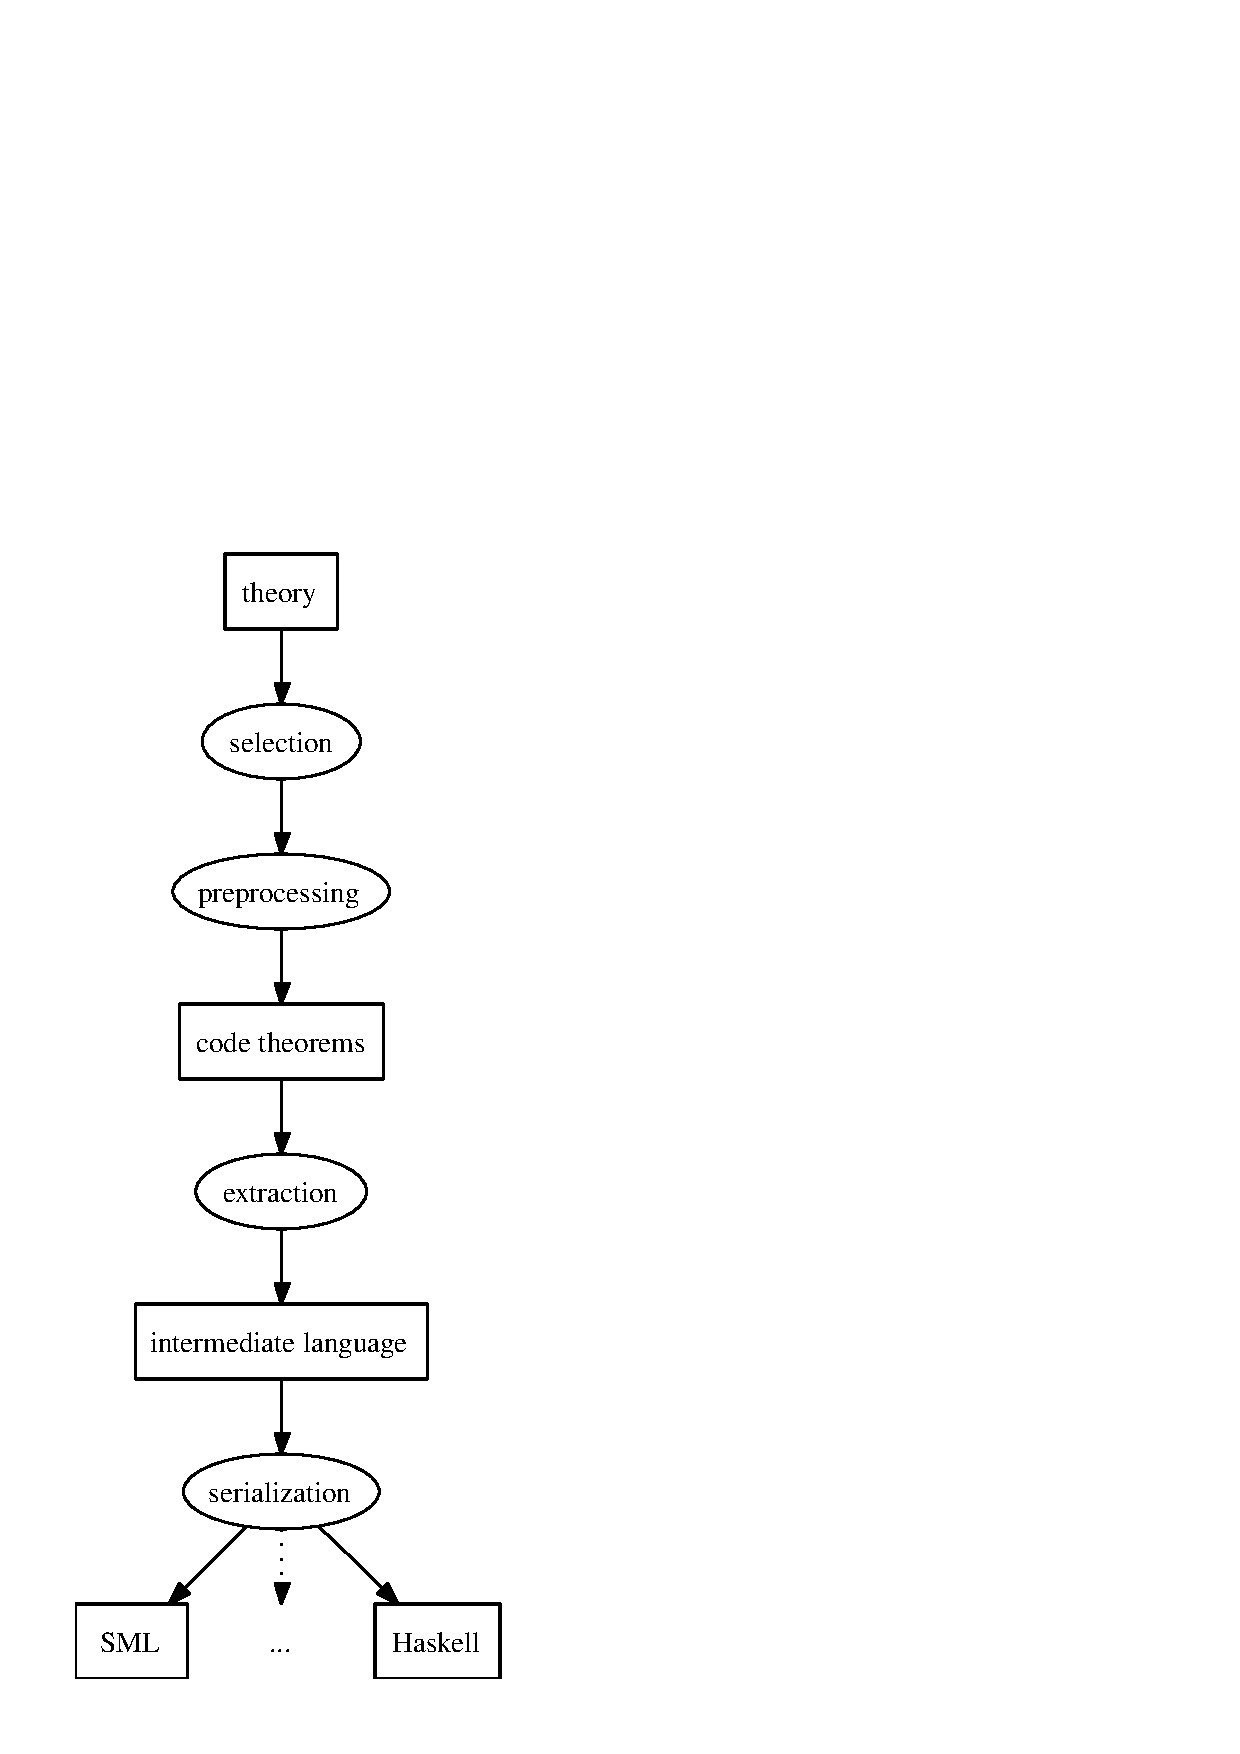
\includegraphics[width=0.7\textwidth]{codegen_process}
    \caption{Code generator architecture}
    \label{fig:arch}
  \end{figure}

  The code generator employs a notion of executability
  for three foundational executable ingredients known
  from functional programming:
  \emph{defining equations}, \emph{datatypes}, and
  \emph{type classes}.  A defining equation as a first approximation
  is a theorem of the form \isa{f\ t\isactrlisub {\isadigit{1}}\ t\isactrlisub {\isadigit{2}}\ {\isasymdots}\ t\isactrlisub n\ {\isasymequiv}\ t}
  (an equation headed by a constant \isa{f} with arguments
  \isa{t\isactrlisub {\isadigit{1}}\ t\isactrlisub {\isadigit{2}}\ {\isasymdots}\ t\isactrlisub n} and right hand side \isa{t}).
  Code generation aims to turn defining equations
  into a functional program.  This is achieved by three major
  components which operate sequentially, i.e. the result of one is
  the input
  of the next in the chain,  see diagram \ref{fig:arch}:

  \begin{itemize}

    \item Out of the vast collection of theorems proven in a
      \qn{theory}, a reasonable subset modelling
      defining equations is \qn{selected}.

    \item On those selected theorems, certain
      transformations are carried out
      (\qn{preprocessing}).  Their purpose is to turn theorems
      representing non- or badly executable
      specifications into equivalent but executable counterparts.
      The result is a structured collection of \qn{code theorems}.

    \item Before the selected defining equations are continued with,
      they can be \qn{preprocessed}, i.e. subjected to theorem
      transformations.  This \qn{preprocessor} is an interface which
      allows to apply
      the full expressiveness of ML-based theorem transformations
      to code generation;  motivating examples are shown below, see
      \secref{sec:preproc}.
      The result of the preprocessing step is a structured collection
      of defining equations.

    \item These defining equations are \qn{translated} to a program
      in an abstract intermediate language.  Think of it as a kind
      of \qt{Mini-Haskell} with four \qn{statements}: \isa{data}
      (for datatypes), \isa{fun} (stemming from defining equations),
      also \isa{class} and \isa{inst} (for type classes).

    \item Finally, the abstract program is \qn{serialised} into concrete
      source code of a target language.

  \end{itemize}

  \noindent From these steps, only the two last are carried out outside the logic;  by
  keeping this layer as thin as possible, the amount of code to trust is
  kept to a minimum.%
\end{isamarkuptext}%
\isamarkuptrue%
%
\isadelimtheory
%
\endisadelimtheory
%
\isatagtheory
\isacommand{end}\isamarkupfalse%
%
\endisatagtheory
{\isafoldtheory}%
%
\isadelimtheory
%
\endisadelimtheory
\isanewline
\end{isabellebody}%
%%% Local Variables:
%%% mode: latex
%%% TeX-master: "root"
%%% End:

%
\begin{isabellebody}%
\def\isabellecontext{Foundations}%
%
\isadelimtheory
%
\endisadelimtheory
%
\isatagtheory
\isacommand{theory}\isamarkupfalse%
\ Foundations\isanewline
\isakeyword{imports}\ Introduction\isanewline
\isakeyword{begin}%
\endisatagtheory
{\isafoldtheory}%
%
\isadelimtheory
%
\endisadelimtheory
%
\isamarkupsection{Code generation foundations \label{sec:foundations}%
}
\isamarkuptrue%
%
\isamarkupsubsection{Code generator architecture \label{sec:architecture}%
}
\isamarkuptrue%
%
\begin{isamarkuptext}%
The code generator is actually a framework consisting of different
  components which can be customised individually.

  Conceptually all components operate on Isabelle's logic framework
  \hyperlink{theory.Pure}{\mbox{\isa{Pure}}}.  Practically, the object logic \hyperlink{theory.HOL}{\mbox{\isa{HOL}}}
  provides the necessary facilities to make use of the code generator,
  mainly since it is an extension of \hyperlink{theory.Pure}{\mbox{\isa{Pure}}}.

  The constellation of the different components is visualized in the
  following picture.

  \begin{figure}[h]
    \includegraphics{architecture}
    \caption{Code generator architecture}
    \label{fig:arch}
  \end{figure}

  \noindent Central to code generation is the notion of \emph{code
  equations}.  A code equation as a first approximation is a theorem
  of the form \isa{f\ t\isactrlisub {\isadigit{1}}\ t\isactrlisub {\isadigit{2}}\ {\isasymdots}\ t\isactrlisub n\ {\isasymequiv}\ t} (an equation headed by a
  constant \isa{f} with arguments \isa{t\isactrlisub {\isadigit{1}}\ t\isactrlisub {\isadigit{2}}\ {\isasymdots}\ t\isactrlisub n} and right
  hand side \isa{t}).

  \begin{itemize}

    \item Starting point of code generation is a collection of (raw)
      code equations in a theory. It is not relevant where they stem
      from, but typically they were either produced by specification
      tools or proved explicitly by the user.
      
    \item These raw code equations can be subjected to theorem
      transformations.  This \qn{preprocessor} (see
      \secref{sec:preproc}) can apply the full expressiveness of
      ML-based theorem transformations to code generation.  The result
      of preprocessing is a structured collection of code equations.

    \item These code equations are \qn{translated} to a program in an
      abstract intermediate language.  Think of it as a kind of
      \qt{Mini-Haskell} with four \qn{statements}: \isa{data} (for
      datatypes), \isa{fun} (stemming from code equations), also
      \isa{class} and \isa{inst} (for type classes).

    \item Finally, the abstract program is \qn{serialised} into
      concrete source code of a target language.  This step only
      produces concrete syntax but does not change the program in
      essence; all conceptual transformations occur in the translation
      step.

  \end{itemize}

  \noindent From these steps, only the last two are carried out
  outside the logic; by keeping this layer as thin as possible, the
  amount of code to trust is kept to a minimum.%
\end{isamarkuptext}%
\isamarkuptrue%
%
\isamarkupsubsection{The preprocessor \label{sec:preproc}%
}
\isamarkuptrue%
%
\begin{isamarkuptext}%
Before selected function theorems are turned into abstract code, a
  chain of definitional transformation steps is carried out:
  \emph{preprocessing}.  The preprocessor consists of two
  components: a \emph{simpset} and \emph{function transformers}.

  The \emph{simpset} can apply the full generality of the Isabelle
  simplifier.  Due to the interpretation of theorems as code
  equations, rewrites are applied to the right hand side and the
  arguments of the left hand side of an equation, but never to the
  constant heading the left hand side.  An important special case are
  \emph{unfold theorems}, which may be declared and removed using the
  \hyperlink{attribute.code-unfold}{\mbox{\isa{code{\isacharunderscore}unfold}}} or \emph{\hyperlink{attribute.code-unfold}{\mbox{\isa{code{\isacharunderscore}unfold}}} del}
  attribute, respectively.

  Some common applications:%
\end{isamarkuptext}%
\isamarkuptrue%
%
\begin{itemize}
%
\begin{isamarkuptext}%
\item replacing non-executable constructs by executable ones:%
\end{isamarkuptext}%
\isamarkuptrue%
%
\isadelimquote
%
\endisadelimquote
%
\isatagquote
\isacommand{lemma}\isamarkupfalse%
\ {\isacharbrackleft}code{\isacharunderscore}unfold{\isacharbrackright}{\isacharcolon}\isanewline
\ \ {\isachardoublequoteopen}x\ {\isasymin}\ set\ xs\ {\isasymlongleftrightarrow}\ List{\isachardot}member\ xs\ x{\isachardoublequoteclose}\ \isacommand{by}\isamarkupfalse%
\ {\isacharparenleft}fact\ in{\isacharunderscore}set{\isacharunderscore}member{\isacharparenright}%
\endisatagquote
{\isafoldquote}%
%
\isadelimquote
%
\endisadelimquote
%
\begin{isamarkuptext}%
\item replacing executable but inconvenient constructs:%
\end{isamarkuptext}%
\isamarkuptrue%
%
\isadelimquote
%
\endisadelimquote
%
\isatagquote
\isacommand{lemma}\isamarkupfalse%
\ {\isacharbrackleft}code{\isacharunderscore}unfold{\isacharbrackright}{\isacharcolon}\isanewline
\ \ {\isachardoublequoteopen}xs\ {\isacharequal}\ {\isacharbrackleft}{\isacharbrackright}\ {\isasymlongleftrightarrow}\ List{\isachardot}null\ xs{\isachardoublequoteclose}\ \isacommand{by}\isamarkupfalse%
\ {\isacharparenleft}fact\ eq{\isacharunderscore}Nil{\isacharunderscore}null{\isacharparenright}%
\endisatagquote
{\isafoldquote}%
%
\isadelimquote
%
\endisadelimquote
%
\begin{isamarkuptext}%
\item eliminating disturbing expressions:%
\end{isamarkuptext}%
\isamarkuptrue%
%
\isadelimquote
%
\endisadelimquote
%
\isatagquote
\isacommand{lemma}\isamarkupfalse%
\ {\isacharbrackleft}code{\isacharunderscore}unfold{\isacharbrackright}{\isacharcolon}\isanewline
\ \ {\isachardoublequoteopen}{\isadigit{1}}\ {\isacharequal}\ Suc\ {\isadigit{0}}{\isachardoublequoteclose}\ \isacommand{by}\isamarkupfalse%
\ {\isacharparenleft}fact\ One{\isacharunderscore}nat{\isacharunderscore}def{\isacharparenright}%
\endisatagquote
{\isafoldquote}%
%
\isadelimquote
%
\endisadelimquote
%
\end{itemize}
%
\begin{isamarkuptext}%
\noindent \emph{Function transformers} provide a very general
  interface, transforming a list of function theorems to another list
  of function theorems, provided that neither the heading constant nor
  its type change.  The \isa{{\isadigit{0}}} / \isa{Suc} pattern
  elimination implemented in theory \hyperlink{theory.Efficient-Nat}{\mbox{\isa{Efficient{\isacharunderscore}Nat}}} (see
  \secref{eff_nat}) uses this interface.

  \noindent The current setup of the preprocessor may be inspected
  using the \indexdef{}{command}{print\_codeproc}\hypertarget{command.print-codeproc}{\hyperlink{command.print-codeproc}{\mbox{\isa{\isacommand{print{\isacharunderscore}codeproc}}}}} command.  \indexdef{}{command}{code\_thms}\hypertarget{command.code-thms}{\hyperlink{command.code-thms}{\mbox{\isa{\isacommand{code{\isacharunderscore}thms}}}}} (see \secref{sec:equations}) provides a convenient
  mechanism to inspect the impact of a preprocessor setup on code
  equations.

  \begin{warn}
    Attribute \hyperlink{attribute.code-unfold}{\mbox{\isa{code{\isacharunderscore}unfold}}} also applies to the
    preprocessor of the ancient \isa{SML\ code\ generator}; in case
    this is not what you intend, use \hyperlink{attribute.code-inline}{\mbox{\isa{code{\isacharunderscore}inline}}} instead.
  \end{warn}%
\end{isamarkuptext}%
\isamarkuptrue%
%
\isamarkupsubsection{Understanding code equations \label{sec:equations}%
}
\isamarkuptrue%
%
\begin{isamarkuptext}%
As told in \secref{sec:principle}, the notion of code equations is
  vital to code generation.  Indeed most problems which occur in
  practice can be resolved by an inspection of the underlying code
  equations.

  It is possible to exchange the default code equations for constants
  by explicitly proving alternative ones:%
\end{isamarkuptext}%
\isamarkuptrue%
%
\isadelimquote
%
\endisadelimquote
%
\isatagquote
\isacommand{lemma}\isamarkupfalse%
\ {\isacharbrackleft}code{\isacharbrackright}{\isacharcolon}\isanewline
\ \ {\isachardoublequoteopen}dequeue\ {\isacharparenleft}AQueue\ xs\ {\isacharbrackleft}{\isacharbrackright}{\isacharparenright}\ {\isacharequal}\isanewline
\ \ \ \ \ {\isacharparenleft}if\ xs\ {\isacharequal}\ {\isacharbrackleft}{\isacharbrackright}\ then\ {\isacharparenleft}None{\isacharcomma}\ AQueue\ {\isacharbrackleft}{\isacharbrackright}\ {\isacharbrackleft}{\isacharbrackright}{\isacharparenright}\isanewline
\ \ \ \ \ \ \ else\ dequeue\ {\isacharparenleft}AQueue\ {\isacharbrackleft}{\isacharbrackright}\ {\isacharparenleft}rev\ xs{\isacharparenright}{\isacharparenright}{\isacharparenright}{\isachardoublequoteclose}\isanewline
\ \ {\isachardoublequoteopen}dequeue\ {\isacharparenleft}AQueue\ xs\ {\isacharparenleft}y\ {\isacharhash}\ ys{\isacharparenright}{\isacharparenright}\ {\isacharequal}\isanewline
\ \ \ \ \ {\isacharparenleft}Some\ y{\isacharcomma}\ AQueue\ xs\ ys{\isacharparenright}{\isachardoublequoteclose}\isanewline
\ \ \isacommand{by}\isamarkupfalse%
\ {\isacharparenleft}cases\ xs{\isacharcomma}\ simp{\isacharunderscore}all{\isacharparenright}\ {\isacharparenleft}cases\ {\isachardoublequoteopen}rev\ xs{\isachardoublequoteclose}{\isacharcomma}\ simp{\isacharunderscore}all{\isacharparenright}%
\endisatagquote
{\isafoldquote}%
%
\isadelimquote
%
\endisadelimquote
%
\begin{isamarkuptext}%
\noindent The annotation \isa{{\isacharbrackleft}code{\isacharbrackright}} is an \isa{attribute}
  which states that the given theorems should be considered as code
  equations for a \isa{fun} statement -- the corresponding constant
  is determined syntactically.  The resulting code:%
\end{isamarkuptext}%
\isamarkuptrue%
%
\isadelimquote
%
\endisadelimquote
%
\isatagquote
%
\begin{isamarkuptext}%
\isatypewriter%
\noindent%
\hspace*{0pt}dequeue ::~forall a.~Example.Queue a -> (Maybe a,~Example.Queue a);\\
\hspace*{0pt}dequeue (Example.AQueue xs (y :~ys)) = (Just y,~Example.AQueue xs ys);\\
\hspace*{0pt}dequeue (Example.AQueue xs []) =\\
\hspace*{0pt} ~(if null xs then (Nothing,~Example.AQueue [] [])\\
\hspace*{0pt} ~~~else Example.dequeue (Example.AQueue [] (reverse xs)));%
\end{isamarkuptext}%
\isamarkuptrue%
%
\endisatagquote
{\isafoldquote}%
%
\isadelimquote
%
\endisadelimquote
%
\begin{isamarkuptext}%
\noindent You may note that the equality test \isa{xs\ {\isacharequal}\ {\isacharbrackleft}{\isacharbrackright}} has
  been replaced by the predicate \isa{List{\isachardot}null\ xs}.  This is due
  to the default setup of the \qn{preprocessor}.

  This possibility to select arbitrary code equations is the key
  technique for program and datatype refinement (see
  \secref{sec:refinement}.

  Due to the preprocessor, there is the distinction of raw code
  equations (before preprocessing) and code equations (after
  preprocessing).

  The first can be listed (among other data) using the \indexdef{}{command}{print\_codesetup}\hypertarget{command.print-codesetup}{\hyperlink{command.print-codesetup}{\mbox{\isa{\isacommand{print{\isacharunderscore}codesetup}}}}} command.

  The code equations after preprocessing are already are blueprint of
  the generated program and can be inspected using the \hyperlink{command.code-thms}{\mbox{\isa{\isacommand{code{\isacharunderscore}thms}}}} command:%
\end{isamarkuptext}%
\isamarkuptrue%
%
\isadelimquote
%
\endisadelimquote
%
\isatagquote
\isacommand{code{\isacharunderscore}thms}\isamarkupfalse%
\ dequeue%
\endisatagquote
{\isafoldquote}%
%
\isadelimquote
%
\endisadelimquote
%
\begin{isamarkuptext}%
\noindent This prints a table with the code equations for \isa{dequeue}, including \emph{all} code equations those equations depend
  on recursively.  These dependencies themselves can be visualized using
  the \indexdef{}{command}{code\_deps}\hypertarget{command.code-deps}{\hyperlink{command.code-deps}{\mbox{\isa{\isacommand{code{\isacharunderscore}deps}}}}} command.%
\end{isamarkuptext}%
\isamarkuptrue%
%
\isamarkupsubsection{Equality%
}
\isamarkuptrue%
%
\begin{isamarkuptext}%
Implementation of equality deserves some attention.  Here an example
  function involving polymorphic equality:%
\end{isamarkuptext}%
\isamarkuptrue%
%
\isadelimquote
%
\endisadelimquote
%
\isatagquote
\isacommand{primrec}\isamarkupfalse%
\ collect{\isacharunderscore}duplicates\ {\isacharcolon}{\isacharcolon}\ {\isachardoublequoteopen}{\isacharprime}a\ list\ {\isasymRightarrow}\ {\isacharprime}a\ list\ {\isasymRightarrow}\ {\isacharprime}a\ list\ {\isasymRightarrow}\ {\isacharprime}a\ list{\isachardoublequoteclose}\ \isakeyword{where}\isanewline
\ \ {\isachardoublequoteopen}collect{\isacharunderscore}duplicates\ xs\ ys\ {\isacharbrackleft}{\isacharbrackright}\ {\isacharequal}\ xs{\isachardoublequoteclose}\isanewline
{\isacharbar}\ {\isachardoublequoteopen}collect{\isacharunderscore}duplicates\ xs\ ys\ {\isacharparenleft}z{\isacharhash}zs{\isacharparenright}\ {\isacharequal}\ {\isacharparenleft}if\ z\ {\isasymin}\ set\ xs\isanewline
\ \ \ \ then\ if\ z\ {\isasymin}\ set\ ys\isanewline
\ \ \ \ \ \ then\ collect{\isacharunderscore}duplicates\ xs\ ys\ zs\isanewline
\ \ \ \ \ \ else\ collect{\isacharunderscore}duplicates\ xs\ {\isacharparenleft}z{\isacharhash}ys{\isacharparenright}\ zs\isanewline
\ \ \ \ else\ collect{\isacharunderscore}duplicates\ {\isacharparenleft}z{\isacharhash}xs{\isacharparenright}\ {\isacharparenleft}z{\isacharhash}ys{\isacharparenright}\ zs{\isacharparenright}{\isachardoublequoteclose}%
\endisatagquote
{\isafoldquote}%
%
\isadelimquote
%
\endisadelimquote
%
\begin{isamarkuptext}%
\noindent During preprocessing, the membership test is rewritten,
  resulting in \isa{List{\isachardot}member}, which itself performs an explicit
  equality check, as can be seen in the corresponding \isa{SML} code:%
\end{isamarkuptext}%
\isamarkuptrue%
%
\isadelimquote
%
\endisadelimquote
%
\isatagquote
%
\begin{isamarkuptext}%
\isatypewriter%
\noindent%
\hspace*{0pt}structure Example :~sig\\
\hspace*{0pt} ~type 'a equal\\
\hspace*{0pt} ~val equal :~'a equal -> 'a -> 'a -> bool\\
\hspace*{0pt} ~val eq :~'a equal -> 'a -> 'a -> bool\\
\hspace*{0pt} ~val member :~'a equal -> 'a list -> 'a -> bool\\
\hspace*{0pt} ~val collect{\char95}duplicates :\\
\hspace*{0pt} ~~~'a equal -> 'a list -> 'a list -> 'a list -> 'a list\\
\hspace*{0pt}end = struct\\
\hspace*{0pt}\\
\hspace*{0pt}type 'a equal = {\char123}equal :~'a -> 'a -> bool{\char125};\\
\hspace*{0pt}val equal = {\char35}equal :~'a equal -> 'a -> 'a -> bool;\\
\hspace*{0pt}\\
\hspace*{0pt}fun eq A{\char95}~a b = equal A{\char95}~a b;\\
\hspace*{0pt}\\
\hspace*{0pt}fun member A{\char95}~[] y = false\\
\hspace*{0pt} ~| member A{\char95}~(x ::~xs) y = eq A{\char95}~x y orelse member A{\char95}~xs y;\\
\hspace*{0pt}\\
\hspace*{0pt}fun collect{\char95}duplicates A{\char95}~xs ys [] = xs\\
\hspace*{0pt} ~| collect{\char95}duplicates A{\char95}~xs ys (z ::~zs) =\\
\hspace*{0pt} ~~~(if member A{\char95}~xs z\\
\hspace*{0pt} ~~~~~then (if member A{\char95}~ys z then collect{\char95}duplicates A{\char95}~xs ys zs\\
\hspace*{0pt} ~~~~~~~~~~~~else collect{\char95}duplicates A{\char95}~xs (z ::~ys) zs)\\
\hspace*{0pt} ~~~~~else collect{\char95}duplicates A{\char95}~(z ::~xs) (z ::~ys) zs);\\
\hspace*{0pt}\\
\hspace*{0pt}end;~(*struct Example*)%
\end{isamarkuptext}%
\isamarkuptrue%
%
\endisatagquote
{\isafoldquote}%
%
\isadelimquote
%
\endisadelimquote
%
\begin{isamarkuptext}%
\noindent Obviously, polymorphic equality is implemented the Haskell
  way using a type class.  How is this achieved?  HOL introduces an
  explicit class \isa{equal} with a corresponding operation \isa{equal{\isacharunderscore}class{\isachardot}equal} such that \isa{equal{\isacharunderscore}class{\isachardot}equal\ {\isacharequal}\ op\ {\isacharequal}}.  The preprocessing
  framework does the rest by propagating the \isa{equal} constraints
  through all dependent code equations.  For datatypes, instances of
  \isa{equal} are implicitly derived when possible.  For other types,
  you may instantiate \isa{equal} manually like any other type class.%
\end{isamarkuptext}%
\isamarkuptrue%
%
\isamarkupsubsection{Explicit partiality \label{sec:partiality}%
}
\isamarkuptrue%
%
\begin{isamarkuptext}%
Partiality usually enters the game by partial patterns, as
  in the following example, again for amortised queues:%
\end{isamarkuptext}%
\isamarkuptrue%
%
\isadelimquote
%
\endisadelimquote
%
\isatagquote
\isacommand{definition}\isamarkupfalse%
\ strict{\isacharunderscore}dequeue\ {\isacharcolon}{\isacharcolon}\ {\isachardoublequoteopen}{\isacharprime}a\ queue\ {\isasymRightarrow}\ {\isacharprime}a\ {\isasymtimes}\ {\isacharprime}a\ queue{\isachardoublequoteclose}\ \isakeyword{where}\isanewline
\ \ {\isachardoublequoteopen}strict{\isacharunderscore}dequeue\ q\ {\isacharequal}\ {\isacharparenleft}case\ dequeue\ q\isanewline
\ \ \ \ of\ {\isacharparenleft}Some\ x{\isacharcomma}\ q{\isacharprime}{\isacharparenright}\ {\isasymRightarrow}\ {\isacharparenleft}x{\isacharcomma}\ q{\isacharprime}{\isacharparenright}{\isacharparenright}{\isachardoublequoteclose}\isanewline
\isanewline
\isacommand{lemma}\isamarkupfalse%
\ strict{\isacharunderscore}dequeue{\isacharunderscore}AQueue\ {\isacharbrackleft}code{\isacharbrackright}{\isacharcolon}\isanewline
\ \ {\isachardoublequoteopen}strict{\isacharunderscore}dequeue\ {\isacharparenleft}AQueue\ xs\ {\isacharparenleft}y\ {\isacharhash}\ ys{\isacharparenright}{\isacharparenright}\ {\isacharequal}\ {\isacharparenleft}y{\isacharcomma}\ AQueue\ xs\ ys{\isacharparenright}{\isachardoublequoteclose}\isanewline
\ \ {\isachardoublequoteopen}strict{\isacharunderscore}dequeue\ {\isacharparenleft}AQueue\ xs\ {\isacharbrackleft}{\isacharbrackright}{\isacharparenright}\ {\isacharequal}\isanewline
\ \ \ \ {\isacharparenleft}case\ rev\ xs\ of\ y\ {\isacharhash}\ ys\ {\isasymRightarrow}\ {\isacharparenleft}y{\isacharcomma}\ AQueue\ {\isacharbrackleft}{\isacharbrackright}\ ys{\isacharparenright}{\isacharparenright}{\isachardoublequoteclose}\isanewline
\ \ \isacommand{by}\isamarkupfalse%
\ {\isacharparenleft}simp{\isacharunderscore}all\ add{\isacharcolon}\ strict{\isacharunderscore}dequeue{\isacharunderscore}def{\isacharparenright}\ {\isacharparenleft}cases\ xs{\isacharcomma}\ simp{\isacharunderscore}all\ split{\isacharcolon}\ list{\isachardot}split{\isacharparenright}%
\endisatagquote
{\isafoldquote}%
%
\isadelimquote
%
\endisadelimquote
%
\begin{isamarkuptext}%
\noindent In the corresponding code, there is no equation
  for the pattern \isa{AQueue\ {\isacharbrackleft}{\isacharbrackright}\ {\isacharbrackleft}{\isacharbrackright}}:%
\end{isamarkuptext}%
\isamarkuptrue%
%
\isadelimquote
%
\endisadelimquote
%
\isatagquote
%
\begin{isamarkuptext}%
\isatypewriter%
\noindent%
\hspace*{0pt}strict{\char95}dequeue ::~forall a.~Example.Queue a -> (a,~Example.Queue a);\\
\hspace*{0pt}strict{\char95}dequeue (Example.AQueue xs []) =\\
\hspace*{0pt} ~let {\char123}\\
\hspace*{0pt} ~~~(y :~ys) = reverse xs;\\
\hspace*{0pt} ~{\char125}~in (y,~Example.AQueue [] ys);\\
\hspace*{0pt}strict{\char95}dequeue (Example.AQueue xs (y :~ys)) = (y,~Example.AQueue xs ys);%
\end{isamarkuptext}%
\isamarkuptrue%
%
\endisatagquote
{\isafoldquote}%
%
\isadelimquote
%
\endisadelimquote
%
\begin{isamarkuptext}%
\noindent In some cases it is desirable to have this
  pseudo-\qt{partiality} more explicitly, e.g.~as follows:%
\end{isamarkuptext}%
\isamarkuptrue%
%
\isadelimquote
%
\endisadelimquote
%
\isatagquote
\isacommand{axiomatization}\isamarkupfalse%
\ empty{\isacharunderscore}queue\ {\isacharcolon}{\isacharcolon}\ {\isacharprime}a\isanewline
\isanewline
\isacommand{definition}\isamarkupfalse%
\ strict{\isacharunderscore}dequeue{\isacharprime}\ {\isacharcolon}{\isacharcolon}\ {\isachardoublequoteopen}{\isacharprime}a\ queue\ {\isasymRightarrow}\ {\isacharprime}a\ {\isasymtimes}\ {\isacharprime}a\ queue{\isachardoublequoteclose}\ \isakeyword{where}\isanewline
\ \ {\isachardoublequoteopen}strict{\isacharunderscore}dequeue{\isacharprime}\ q\ {\isacharequal}\ {\isacharparenleft}case\ dequeue\ q\ of\ {\isacharparenleft}Some\ x{\isacharcomma}\ q{\isacharprime}{\isacharparenright}\ {\isasymRightarrow}\ {\isacharparenleft}x{\isacharcomma}\ q{\isacharprime}{\isacharparenright}\ {\isacharbar}\ {\isacharunderscore}\ {\isasymRightarrow}\ empty{\isacharunderscore}queue{\isacharparenright}{\isachardoublequoteclose}\isanewline
\isanewline
\isacommand{lemma}\isamarkupfalse%
\ strict{\isacharunderscore}dequeue{\isacharprime}{\isacharunderscore}AQueue\ {\isacharbrackleft}code{\isacharbrackright}{\isacharcolon}\isanewline
\ \ {\isachardoublequoteopen}strict{\isacharunderscore}dequeue{\isacharprime}\ {\isacharparenleft}AQueue\ xs\ {\isacharbrackleft}{\isacharbrackright}{\isacharparenright}\ {\isacharequal}\ {\isacharparenleft}if\ xs\ {\isacharequal}\ {\isacharbrackleft}{\isacharbrackright}\ then\ empty{\isacharunderscore}queue\isanewline
\ \ \ \ \ else\ strict{\isacharunderscore}dequeue{\isacharprime}\ {\isacharparenleft}AQueue\ {\isacharbrackleft}{\isacharbrackright}\ {\isacharparenleft}rev\ xs{\isacharparenright}{\isacharparenright}{\isacharparenright}{\isachardoublequoteclose}\isanewline
\ \ {\isachardoublequoteopen}strict{\isacharunderscore}dequeue{\isacharprime}\ {\isacharparenleft}AQueue\ xs\ {\isacharparenleft}y\ {\isacharhash}\ ys{\isacharparenright}{\isacharparenright}\ {\isacharequal}\isanewline
\ \ \ \ \ {\isacharparenleft}y{\isacharcomma}\ AQueue\ xs\ ys{\isacharparenright}{\isachardoublequoteclose}\isanewline
\ \ \isacommand{by}\isamarkupfalse%
\ {\isacharparenleft}simp{\isacharunderscore}all\ add{\isacharcolon}\ strict{\isacharunderscore}dequeue{\isacharprime}{\isacharunderscore}def\ split{\isacharcolon}\ list{\isachardot}splits{\isacharparenright}%
\endisatagquote
{\isafoldquote}%
%
\isadelimquote
%
\endisadelimquote
%
\begin{isamarkuptext}%
Observe that on the right hand side of the definition of \isa{strict{\isacharunderscore}dequeue{\isacharprime}}, the unspecified constant \isa{empty{\isacharunderscore}queue} occurs.

  Normally, if constants without any code equations occur in a
  program, the code generator complains (since in most cases this is
  indeed an error).  But such constants can also be thought
  of as function definitions which always fail,
  since there is never a successful pattern match on the left hand
  side.  In order to categorise a constant into that category
  explicitly, use \indexdef{}{command}{code\_abort}\hypertarget{command.code-abort}{\hyperlink{command.code-abort}{\mbox{\isa{\isacommand{code{\isacharunderscore}abort}}}}}:%
\end{isamarkuptext}%
\isamarkuptrue%
%
\isadelimquote
%
\endisadelimquote
%
\isatagquote
\isacommand{code{\isacharunderscore}abort}\isamarkupfalse%
\ empty{\isacharunderscore}queue%
\endisatagquote
{\isafoldquote}%
%
\isadelimquote
%
\endisadelimquote
%
\begin{isamarkuptext}%
\noindent Then the code generator will just insert an error or
  exception at the appropriate position:%
\end{isamarkuptext}%
\isamarkuptrue%
%
\isadelimquote
%
\endisadelimquote
%
\isatagquote
%
\begin{isamarkuptext}%
\isatypewriter%
\noindent%
\hspace*{0pt}empty{\char95}queue ::~forall a.~a;\\
\hspace*{0pt}empty{\char95}queue = error {\char34}empty{\char95}queue{\char34};\\
\hspace*{0pt}\\
\hspace*{0pt}strict{\char95}dequeue ::~forall a.~Example.Queue a -> (a,~Example.Queue a);\\
\hspace*{0pt}strict{\char95}dequeue (Example.AQueue xs (y :~ys)) = (y,~Example.AQueue xs ys);\\
\hspace*{0pt}strict{\char95}dequeue (Example.AQueue xs []) =\\
\hspace*{0pt} ~(if null xs then Example.empty{\char95}queue\\
\hspace*{0pt} ~~~else Example.strict{\char95}dequeue (Example.AQueue [] (reverse xs)));%
\end{isamarkuptext}%
\isamarkuptrue%
%
\endisatagquote
{\isafoldquote}%
%
\isadelimquote
%
\endisadelimquote
%
\begin{isamarkuptext}%
\noindent This feature however is rarely needed in practice.  Note
  also that the HOL default setup already declares \isa{undefined}
  as \hyperlink{command.code-abort}{\mbox{\isa{\isacommand{code{\isacharunderscore}abort}}}}, which is most likely to be used in such
  situations.%
\end{isamarkuptext}%
\isamarkuptrue%
%
\isamarkupsubsection{If something goes utterly wrong \label{sec:utterly_wrong}%
}
\isamarkuptrue%
%
\begin{isamarkuptext}%
Under certain circumstances, the code generator fails to produce
  code entirely.  To debug these, the following hints may prove
  helpful:

  \begin{description}

    \ditem{\emph{Check with a different target language}.}  Sometimes
      the situation gets more clear if you switch to another target
      language; the code generated there might give some hints what
      prevents the code generator to produce code for the desired
      language.

    \ditem{\emph{Inspect code equations}.}  Code equations are the central
      carrier of code generation.  Most problems occuring while generation
      code can be traced to single equations which are printed as part of
      the error message.  A closer inspection of those may offer the key
      for solving issues (cf.~\secref{sec:equations}).

    \ditem{\emph{Inspect preprocessor setup}.}  The preprocessor might
      transform code equations unexpectedly; to understand an
      inspection of its setup is necessary (cf.~\secref{sec:preproc}).

    \ditem{\emph{Generate exceptions}.}  If the code generator
      complains about missing code equations, in can be helpful to
      implement the offending constants as exceptions
      (cf.~\secref{sec:partiality}); this allows at least for a formal
      generation of code, whose inspection may then give clues what is
      wrong.

    \ditem{\emph{Remove offending code equations}.}  If code
      generation is prevented by just a single equation, this can be
      removed (cf.~\secref{sec:equations}) to allow formal code
      generation, whose result in turn can be used to trace the
      problem.  The most prominent case here are mismatches in type
      class signatures (\qt{wellsortedness error}).

  \end{description}%
\end{isamarkuptext}%
\isamarkuptrue%
%
\isadelimtheory
%
\endisadelimtheory
%
\isatagtheory
\isacommand{end}\isamarkupfalse%
%
\endisatagtheory
{\isafoldtheory}%
%
\isadelimtheory
%
\endisadelimtheory
\isanewline
\end{isabellebody}%
%%% Local Variables:
%%% mode: latex
%%% TeX-master: "root"
%%% End:

%
\begin{isabellebody}%
\def\isabellecontext{Refinement}%
%
\isadelimtheory
%
\endisadelimtheory
%
\isatagtheory
\isacommand{theory}\isamarkupfalse%
\ Refinement\isanewline
\isakeyword{imports}\ Setup\isanewline
\isakeyword{begin}%
\endisatagtheory
{\isafoldtheory}%
%
\isadelimtheory
%
\endisadelimtheory
%
\isamarkupsection{Program and datatype refinement \label{sec:refinement}%
}
\isamarkuptrue%
%
\begin{isamarkuptext}%
Code generation by shallow embedding (cf.~\secref{sec:principle})
  allows to choose code equations and datatype constructors freely,
  given that some very basic syntactic properties are met; this
  flexibility opens up mechanisms for refinement which allow to extend
  the scope and quality of generated code dramatically.%
\end{isamarkuptext}%
\isamarkuptrue%
%
\isamarkupsubsection{Program refinement%
}
\isamarkuptrue%
%
\begin{isamarkuptext}%
Program refinement works by choosing appropriate code equations
  explicitly (cf.~\label{sec:equations}); as example, we use Fibonacci
  numbers:%
\end{isamarkuptext}%
\isamarkuptrue%
%
\isadelimquote
%
\endisadelimquote
%
\isatagquote
\isacommand{fun}\isamarkupfalse%
\ fib\ {\isacharcolon}{\isacharcolon}\ {\isachardoublequoteopen}nat\ {\isasymRightarrow}\ nat{\isachardoublequoteclose}\ \isakeyword{where}\isanewline
\ \ \ \ {\isachardoublequoteopen}fib\ {\isadigit{0}}\ {\isacharequal}\ {\isadigit{0}}{\isachardoublequoteclose}\isanewline
\ \ {\isacharbar}\ {\isachardoublequoteopen}fib\ {\isacharparenleft}Suc\ {\isadigit{0}}{\isacharparenright}\ {\isacharequal}\ Suc\ {\isadigit{0}}{\isachardoublequoteclose}\isanewline
\ \ {\isacharbar}\ {\isachardoublequoteopen}fib\ {\isacharparenleft}Suc\ {\isacharparenleft}Suc\ n{\isacharparenright}{\isacharparenright}\ {\isacharequal}\ fib\ n\ {\isacharplus}\ fib\ {\isacharparenleft}Suc\ n{\isacharparenright}{\isachardoublequoteclose}%
\endisatagquote
{\isafoldquote}%
%
\isadelimquote
%
\endisadelimquote
%
\begin{isamarkuptext}%
\noindent The runtime of the corresponding code grows exponential due
  to two recursive calls:%
\end{isamarkuptext}%
\isamarkuptrue%
%
\isadelimquote
%
\endisadelimquote
%
\isatagquote
%
\begin{isamarkuptext}%
\isatypewriter%
\noindent%
\hspace*{0pt}fib ::~Example.Nat -> Example.Nat;\\
\hspace*{0pt}fib Example.Zero{\char95}nat = Example.Zero{\char95}nat;\\
\hspace*{0pt}fib (Example.Suc Example.Zero{\char95}nat) = Example.Suc Example.Zero{\char95}nat;\\
\hspace*{0pt}fib (Example.Suc (Example.Suc n)) =\\
\hspace*{0pt} ~Example.plus{\char95}nat (Example.fib n) (Example.fib (Example.Suc n));%
\end{isamarkuptext}%
\isamarkuptrue%
%
\endisatagquote
{\isafoldquote}%
%
\isadelimquote
%
\endisadelimquote
%
\begin{isamarkuptext}%
\noindent A more efficient implementation would use dynamic
  programming, e.g.~sharing of common intermediate results between
  recursive calls.  This idea is expressed by an auxiliary operation
  which computes a Fibonacci number and its successor simultaneously:%
\end{isamarkuptext}%
\isamarkuptrue%
%
\isadelimquote
%
\endisadelimquote
%
\isatagquote
\isacommand{definition}\isamarkupfalse%
\ fib{\isacharunderscore}step\ {\isacharcolon}{\isacharcolon}\ {\isachardoublequoteopen}nat\ {\isasymRightarrow}\ nat\ {\isasymtimes}\ nat{\isachardoublequoteclose}\ \isakeyword{where}\isanewline
\ \ {\isachardoublequoteopen}fib{\isacharunderscore}step\ n\ {\isacharequal}\ {\isacharparenleft}fib\ {\isacharparenleft}Suc\ n{\isacharparenright}{\isacharcomma}\ fib\ n{\isacharparenright}{\isachardoublequoteclose}%
\endisatagquote
{\isafoldquote}%
%
\isadelimquote
%
\endisadelimquote
%
\begin{isamarkuptext}%
\noindent This operation can be implemented by recursion using
  dynamic programming:%
\end{isamarkuptext}%
\isamarkuptrue%
%
\isadelimquote
%
\endisadelimquote
%
\isatagquote
\isacommand{lemma}\isamarkupfalse%
\ {\isacharbrackleft}code{\isacharbrackright}{\isacharcolon}\isanewline
\ \ {\isachardoublequoteopen}fib{\isacharunderscore}step\ {\isadigit{0}}\ {\isacharequal}\ {\isacharparenleft}Suc\ {\isadigit{0}}{\isacharcomma}\ {\isadigit{0}}{\isacharparenright}{\isachardoublequoteclose}\isanewline
\ \ {\isachardoublequoteopen}fib{\isacharunderscore}step\ {\isacharparenleft}Suc\ n{\isacharparenright}\ {\isacharequal}\ {\isacharparenleft}let\ {\isacharparenleft}m{\isacharcomma}\ q{\isacharparenright}\ {\isacharequal}\ fib{\isacharunderscore}step\ n\ in\ {\isacharparenleft}m\ {\isacharplus}\ q{\isacharcomma}\ m{\isacharparenright}{\isacharparenright}{\isachardoublequoteclose}\isanewline
\ \ \isacommand{by}\isamarkupfalse%
\ {\isacharparenleft}simp{\isacharunderscore}all\ add{\isacharcolon}\ fib{\isacharunderscore}step{\isacharunderscore}def{\isacharparenright}%
\endisatagquote
{\isafoldquote}%
%
\isadelimquote
%
\endisadelimquote
%
\begin{isamarkuptext}%
\noindent What remains is to implement \isa{fib} by \isa{fib{\isacharunderscore}step} as follows:%
\end{isamarkuptext}%
\isamarkuptrue%
%
\isadelimquote
%
\endisadelimquote
%
\isatagquote
\isacommand{lemma}\isamarkupfalse%
\ {\isacharbrackleft}code{\isacharbrackright}{\isacharcolon}\isanewline
\ \ {\isachardoublequoteopen}fib\ {\isadigit{0}}\ {\isacharequal}\ {\isadigit{0}}{\isachardoublequoteclose}\isanewline
\ \ {\isachardoublequoteopen}fib\ {\isacharparenleft}Suc\ n{\isacharparenright}\ {\isacharequal}\ fst\ {\isacharparenleft}fib{\isacharunderscore}step\ n{\isacharparenright}{\isachardoublequoteclose}\isanewline
\ \ \isacommand{by}\isamarkupfalse%
\ {\isacharparenleft}simp{\isacharunderscore}all\ add{\isacharcolon}\ fib{\isacharunderscore}step{\isacharunderscore}def{\isacharparenright}%
\endisatagquote
{\isafoldquote}%
%
\isadelimquote
%
\endisadelimquote
%
\begin{isamarkuptext}%
\noindent The resulting code shows only linear growth of runtime:%
\end{isamarkuptext}%
\isamarkuptrue%
%
\isadelimquote
%
\endisadelimquote
%
\isatagquote
%
\begin{isamarkuptext}%
\isatypewriter%
\noindent%
\hspace*{0pt}fib{\char95}step ::~Example.Nat -> (Example.Nat,~Example.Nat);\\
\hspace*{0pt}fib{\char95}step (Example.Suc n) =\\
\hspace*{0pt} ~let {\char123}\\
\hspace*{0pt} ~~~(m,~q) = Example.fib{\char95}step n;\\
\hspace*{0pt} ~{\char125}~in (Example.plus{\char95}nat m q,~m);\\
\hspace*{0pt}fib{\char95}step Example.Zero{\char95}nat =\\
\hspace*{0pt} ~(Example.Suc Example.Zero{\char95}nat,~Example.Zero{\char95}nat);\\
\hspace*{0pt}\\
\hspace*{0pt}fib ::~Example.Nat -> Example.Nat;\\
\hspace*{0pt}fib (Example.Suc n) = fst (Example.fib{\char95}step n);\\
\hspace*{0pt}fib Example.Zero{\char95}nat = Example.Zero{\char95}nat;%
\end{isamarkuptext}%
\isamarkuptrue%
%
\endisatagquote
{\isafoldquote}%
%
\isadelimquote
%
\endisadelimquote
%
\isamarkupsubsection{Datatype refinement%
}
\isamarkuptrue%
%
\begin{isamarkuptext}%
Selecting specific code equations \emph{and} datatype constructors
  leads to datatype refinement.  As an example, we will develop an
  alternative representation of the queue example given in
  \secref{sec:queue_example}.  The amortised representation is
  convenient for generating code but exposes its \qt{implementation}
  details, which may be cumbersome when proving theorems about it.
  Therefore, here is a simple, straightforward representation of
  queues:%
\end{isamarkuptext}%
\isamarkuptrue%
%
\isadelimquote
%
\endisadelimquote
%
\isatagquote
\isacommand{datatype}\isamarkupfalse%
\ {\isacharprime}a\ queue\ {\isacharequal}\ Queue\ {\isachardoublequoteopen}{\isacharprime}a\ list{\isachardoublequoteclose}\isanewline
\isanewline
\isacommand{definition}\isamarkupfalse%
\ empty\ {\isacharcolon}{\isacharcolon}\ {\isachardoublequoteopen}{\isacharprime}a\ queue{\isachardoublequoteclose}\ \isakeyword{where}\isanewline
\ \ {\isachardoublequoteopen}empty\ {\isacharequal}\ Queue\ {\isacharbrackleft}{\isacharbrackright}{\isachardoublequoteclose}\isanewline
\isanewline
\isacommand{primrec}\isamarkupfalse%
\ enqueue\ {\isacharcolon}{\isacharcolon}\ {\isachardoublequoteopen}{\isacharprime}a\ {\isasymRightarrow}\ {\isacharprime}a\ queue\ {\isasymRightarrow}\ {\isacharprime}a\ queue{\isachardoublequoteclose}\ \isakeyword{where}\isanewline
\ \ {\isachardoublequoteopen}enqueue\ x\ {\isacharparenleft}Queue\ xs{\isacharparenright}\ {\isacharequal}\ Queue\ {\isacharparenleft}xs\ {\isacharat}\ {\isacharbrackleft}x{\isacharbrackright}{\isacharparenright}{\isachardoublequoteclose}\isanewline
\isanewline
\isacommand{fun}\isamarkupfalse%
\ dequeue\ {\isacharcolon}{\isacharcolon}\ {\isachardoublequoteopen}{\isacharprime}a\ queue\ {\isasymRightarrow}\ {\isacharprime}a\ option\ {\isasymtimes}\ {\isacharprime}a\ queue{\isachardoublequoteclose}\ \isakeyword{where}\isanewline
\ \ \ \ {\isachardoublequoteopen}dequeue\ {\isacharparenleft}Queue\ {\isacharbrackleft}{\isacharbrackright}{\isacharparenright}\ {\isacharequal}\ {\isacharparenleft}None{\isacharcomma}\ Queue\ {\isacharbrackleft}{\isacharbrackright}{\isacharparenright}{\isachardoublequoteclose}\isanewline
\ \ {\isacharbar}\ {\isachardoublequoteopen}dequeue\ {\isacharparenleft}Queue\ {\isacharparenleft}x\ {\isacharhash}\ xs{\isacharparenright}{\isacharparenright}\ {\isacharequal}\ {\isacharparenleft}Some\ x{\isacharcomma}\ Queue\ xs{\isacharparenright}{\isachardoublequoteclose}%
\endisatagquote
{\isafoldquote}%
%
\isadelimquote
%
\endisadelimquote
%
\begin{isamarkuptext}%
\noindent This we can use directly for proving;  for executing,
  we provide an alternative characterisation:%
\end{isamarkuptext}%
\isamarkuptrue%
%
\isadelimquote
%
\endisadelimquote
%
\isatagquote
\isacommand{definition}\isamarkupfalse%
\ AQueue\ {\isacharcolon}{\isacharcolon}\ {\isachardoublequoteopen}{\isacharprime}a\ list\ {\isasymRightarrow}\ {\isacharprime}a\ list\ {\isasymRightarrow}\ {\isacharprime}a\ queue{\isachardoublequoteclose}\ \isakeyword{where}\isanewline
\ \ {\isachardoublequoteopen}AQueue\ xs\ ys\ {\isacharequal}\ Queue\ {\isacharparenleft}ys\ {\isacharat}\ rev\ xs{\isacharparenright}{\isachardoublequoteclose}\isanewline
\isanewline
\isacommand{code{\isacharunderscore}datatype}\isamarkupfalse%
\ AQueue%
\endisatagquote
{\isafoldquote}%
%
\isadelimquote
%
\endisadelimquote
%
\begin{isamarkuptext}%
\noindent Here we define a \qt{constructor} \isa{AQueue} which
  is defined in terms of \isa{Queue} and interprets its arguments
  according to what the \emph{content} of an amortised queue is supposed
  to be.

  The prerequisite for datatype constructors is only syntactical: a
  constructor must be of type \isa{{\isasymtau}\ {\isacharequal}\ {\isasymdots}\ {\isasymRightarrow}\ {\isasymkappa}\ {\isasymalpha}\isactrlisub {\isadigit{1}}\ {\isasymdots}\ {\isasymalpha}\isactrlisub n} where \isa{{\isacharbraceleft}{\isasymalpha}\isactrlisub {\isadigit{1}}{\isacharcomma}\ {\isasymdots}{\isacharcomma}\ {\isasymalpha}\isactrlisub n{\isacharbraceright}} is exactly the set of \emph{all} type variables in
  \isa{{\isasymtau}}; then \isa{{\isasymkappa}} is its corresponding datatype.  The
  HOL datatype package by default registers any new datatype with its
  constructors, but this may be changed using \indexdef{}{command}{code\_datatype}\hypertarget{command.code-datatype}{\hyperlink{command.code-datatype}{\mbox{\isa{\isacommand{code{\isacharunderscore}datatype}}}}}; the currently chosen constructors can be inspected
  using the \hyperlink{command.print-codesetup}{\mbox{\isa{\isacommand{print{\isacharunderscore}codesetup}}}} command.

  Equipped with this, we are able to prove the following equations
  for our primitive queue operations which \qt{implement} the simple
  queues in an amortised fashion:%
\end{isamarkuptext}%
\isamarkuptrue%
%
\isadelimquote
%
\endisadelimquote
%
\isatagquote
\isacommand{lemma}\isamarkupfalse%
\ empty{\isacharunderscore}AQueue\ {\isacharbrackleft}code{\isacharbrackright}{\isacharcolon}\isanewline
\ \ {\isachardoublequoteopen}empty\ {\isacharequal}\ AQueue\ {\isacharbrackleft}{\isacharbrackright}\ {\isacharbrackleft}{\isacharbrackright}{\isachardoublequoteclose}\isanewline
\ \ \isacommand{unfolding}\isamarkupfalse%
\ AQueue{\isacharunderscore}def\ empty{\isacharunderscore}def\ \isacommand{by}\isamarkupfalse%
\ simp\isanewline
\isanewline
\isacommand{lemma}\isamarkupfalse%
\ enqueue{\isacharunderscore}AQueue\ {\isacharbrackleft}code{\isacharbrackright}{\isacharcolon}\isanewline
\ \ {\isachardoublequoteopen}enqueue\ x\ {\isacharparenleft}AQueue\ xs\ ys{\isacharparenright}\ {\isacharequal}\ AQueue\ {\isacharparenleft}x\ {\isacharhash}\ xs{\isacharparenright}\ ys{\isachardoublequoteclose}\isanewline
\ \ \isacommand{unfolding}\isamarkupfalse%
\ AQueue{\isacharunderscore}def\ \isacommand{by}\isamarkupfalse%
\ simp\isanewline
\isanewline
\isacommand{lemma}\isamarkupfalse%
\ dequeue{\isacharunderscore}AQueue\ {\isacharbrackleft}code{\isacharbrackright}{\isacharcolon}\isanewline
\ \ {\isachardoublequoteopen}dequeue\ {\isacharparenleft}AQueue\ xs\ {\isacharbrackleft}{\isacharbrackright}{\isacharparenright}\ {\isacharequal}\isanewline
\ \ \ \ {\isacharparenleft}if\ xs\ {\isacharequal}\ {\isacharbrackleft}{\isacharbrackright}\ then\ {\isacharparenleft}None{\isacharcomma}\ AQueue\ {\isacharbrackleft}{\isacharbrackright}\ {\isacharbrackleft}{\isacharbrackright}{\isacharparenright}\isanewline
\ \ \ \ else\ dequeue\ {\isacharparenleft}AQueue\ {\isacharbrackleft}{\isacharbrackright}\ {\isacharparenleft}rev\ xs{\isacharparenright}{\isacharparenright}{\isacharparenright}{\isachardoublequoteclose}\isanewline
\ \ {\isachardoublequoteopen}dequeue\ {\isacharparenleft}AQueue\ xs\ {\isacharparenleft}y\ {\isacharhash}\ ys{\isacharparenright}{\isacharparenright}\ {\isacharequal}\ {\isacharparenleft}Some\ y{\isacharcomma}\ AQueue\ xs\ ys{\isacharparenright}{\isachardoublequoteclose}\isanewline
\ \ \isacommand{unfolding}\isamarkupfalse%
\ AQueue{\isacharunderscore}def\ \isacommand{by}\isamarkupfalse%
\ simp{\isacharunderscore}all%
\endisatagquote
{\isafoldquote}%
%
\isadelimquote
%
\endisadelimquote
%
\begin{isamarkuptext}%
\noindent For completeness, we provide a substitute for the
  \isa{case} combinator on queues:%
\end{isamarkuptext}%
\isamarkuptrue%
%
\isadelimquote
%
\endisadelimquote
%
\isatagquote
\isacommand{lemma}\isamarkupfalse%
\ queue{\isacharunderscore}case{\isacharunderscore}AQueue\ {\isacharbrackleft}code{\isacharbrackright}{\isacharcolon}\isanewline
\ \ {\isachardoublequoteopen}queue{\isacharunderscore}case\ f\ {\isacharparenleft}AQueue\ xs\ ys{\isacharparenright}\ {\isacharequal}\ f\ {\isacharparenleft}ys\ {\isacharat}\ rev\ xs{\isacharparenright}{\isachardoublequoteclose}\isanewline
\ \ \isacommand{unfolding}\isamarkupfalse%
\ AQueue{\isacharunderscore}def\ \isacommand{by}\isamarkupfalse%
\ simp%
\endisatagquote
{\isafoldquote}%
%
\isadelimquote
%
\endisadelimquote
%
\begin{isamarkuptext}%
\noindent The resulting code looks as expected:%
\end{isamarkuptext}%
\isamarkuptrue%
%
\isadelimquote
%
\endisadelimquote
%
\isatagquote
%
\begin{isamarkuptext}%
\isatypewriter%
\noindent%
\hspace*{0pt}structure Example :~sig\\
\hspace*{0pt} ~val id :~'a -> 'a\\
\hspace*{0pt} ~val fold :~('a -> 'b -> 'b) -> 'a list -> 'b -> 'b\\
\hspace*{0pt} ~val rev :~'a list -> 'a list\\
\hspace*{0pt} ~val null :~'a list -> bool\\
\hspace*{0pt} ~datatype 'a queue = AQueue of 'a list * 'a list\\
\hspace*{0pt} ~val empty :~'a queue\\
\hspace*{0pt} ~val dequeue :~'a queue -> 'a option * 'a queue\\
\hspace*{0pt} ~val enqueue :~'a -> 'a queue -> 'a queue\\
\hspace*{0pt}end = struct\\
\hspace*{0pt}\\
\hspace*{0pt}fun id x = (fn xa => xa) x;\\
\hspace*{0pt}\\
\hspace*{0pt}fun fold f [] = id\\
\hspace*{0pt} ~| fold f (x ::~xs) = fold f xs o f x;\\
\hspace*{0pt}\\
\hspace*{0pt}fun rev xs = fold (fn a => fn b => a ::~b) xs [];\\
\hspace*{0pt}\\
\hspace*{0pt}fun null [] = true\\
\hspace*{0pt} ~| null (x ::~xs) = false;\\
\hspace*{0pt}\\
\hspace*{0pt}datatype 'a queue = AQueue of 'a list * 'a list;\\
\hspace*{0pt}\\
\hspace*{0pt}val empty :~'a queue = AQueue ([],~[]);\\
\hspace*{0pt}\\
\hspace*{0pt}fun dequeue (AQueue (xs,~y ::~ys)) = (SOME y,~AQueue (xs,~ys))\\
\hspace*{0pt} ~| dequeue (AQueue (xs,~[])) =\\
\hspace*{0pt} ~~~(if null xs then (NONE,~AQueue ([],~[]))\\
\hspace*{0pt} ~~~~~else dequeue (AQueue ([],~rev xs)));\\
\hspace*{0pt}\\
\hspace*{0pt}fun enqueue x (AQueue (xs,~ys)) = AQueue (x ::~xs,~ys);\\
\hspace*{0pt}\\
\hspace*{0pt}end;~(*struct Example*)%
\end{isamarkuptext}%
\isamarkuptrue%
%
\endisatagquote
{\isafoldquote}%
%
\isadelimquote
%
\endisadelimquote
%
\begin{isamarkuptext}%
The same techniques can also be applied to types which are not
  specified as datatypes, e.g.~type \isa{int} is originally specified
  as quotient type by means of \indexdef{}{command}{typedef}\hypertarget{command.typedef}{\hyperlink{command.typedef}{\mbox{\isa{\isacommand{typedef}}}}}, but for code
  generation constants allowing construction of binary numeral values
  are used as constructors for \isa{int}.

  This approach however fails if the representation of a type demands
  invariants; this issue is discussed in the next section.%
\end{isamarkuptext}%
\isamarkuptrue%
%
\isamarkupsubsection{Datatype refinement involving invariants%
}
\isamarkuptrue%
%
\begin{isamarkuptext}%
Datatype representation involving invariants require a dedicated
  setup for the type and its primitive operations.  As a running
  example, we implement a type \isa{{\isacharprime}a\ dlist} of list consisting
  of distinct elements.

  The first step is to decide on which representation the abstract
  type (in our example \isa{{\isacharprime}a\ dlist}) should be implemented.
  Here we choose \isa{{\isacharprime}a\ list}.  Then a conversion from the concrete
  type to the abstract type must be specified, here:%
\end{isamarkuptext}%
\isamarkuptrue%
%
\isadelimquote
%
\endisadelimquote
%
\isatagquote
%
\begin{isamarkuptext}%
\isa{Dlist\ {\isasymColon}\ {\isacharprime}a\ list\ {\isasymRightarrow}\ {\isacharprime}a\ dlist}%
\end{isamarkuptext}%
\isamarkuptrue%
%
\endisatagquote
{\isafoldquote}%
%
\isadelimquote
%
\endisadelimquote
%
\begin{isamarkuptext}%
\noindent Next follows the specification of a suitable \emph{projection},
  i.e.~a conversion from abstract to concrete type:%
\end{isamarkuptext}%
\isamarkuptrue%
%
\isadelimquote
%
\endisadelimquote
%
\isatagquote
%
\begin{isamarkuptext}%
\isa{list{\isacharunderscore}of{\isacharunderscore}dlist\ {\isasymColon}\ {\isacharprime}a\ dlist\ {\isasymRightarrow}\ {\isacharprime}a\ list}%
\end{isamarkuptext}%
\isamarkuptrue%
%
\endisatagquote
{\isafoldquote}%
%
\isadelimquote
%
\endisadelimquote
%
\begin{isamarkuptext}%
\noindent This projection must be specified such that the following
  \emph{abstract datatype certificate} can be proven:%
\end{isamarkuptext}%
\isamarkuptrue%
%
\isadelimquote
%
\endisadelimquote
%
\isatagquote
\isacommand{lemma}\isamarkupfalse%
\ {\isacharbrackleft}code\ abstype{\isacharbrackright}{\isacharcolon}\isanewline
\ \ {\isachardoublequoteopen}Dlist\ {\isacharparenleft}list{\isacharunderscore}of{\isacharunderscore}dlist\ dxs{\isacharparenright}\ {\isacharequal}\ dxs{\isachardoublequoteclose}\isanewline
\ \ \isacommand{by}\isamarkupfalse%
\ {\isacharparenleft}fact\ Dlist{\isacharunderscore}list{\isacharunderscore}of{\isacharunderscore}dlist{\isacharparenright}%
\endisatagquote
{\isafoldquote}%
%
\isadelimquote
%
\endisadelimquote
%
\begin{isamarkuptext}%
\noindent Note that so far the invariant on representations
  (\isa{distinct\ {\isasymColon}\ {\isacharprime}a\ list\ {\isasymRightarrow}\ bool}) has never been mentioned explicitly:
  the invariant is only referred to implicitly: all values in
  set \isa{{\isacharbraceleft}xs{\isachardot}\ list{\isacharunderscore}of{\isacharunderscore}dlist\ {\isacharparenleft}Dlist\ xs{\isacharparenright}\ {\isacharequal}\ xs{\isacharbraceright}} are invariant,
  and in our example this is exactly \isa{{\isacharbraceleft}xs{\isachardot}\ distinct\ xs{\isacharbraceright}}.
  
  The primitive operations on \isa{{\isacharprime}a\ dlist} are specified
  indirectly using the projection \isa{list{\isacharunderscore}of{\isacharunderscore}dlist}.  For
  the empty \isa{dlist}, \isa{Dlist{\isachardot}empty}, we finally want
  the code equation%
\end{isamarkuptext}%
\isamarkuptrue%
%
\isadelimquote
%
\endisadelimquote
%
\isatagquote
%
\begin{isamarkuptext}%
\isa{Dlist{\isachardot}empty\ {\isacharequal}\ Dlist\ {\isacharbrackleft}{\isacharbrackright}}%
\end{isamarkuptext}%
\isamarkuptrue%
%
\endisatagquote
{\isafoldquote}%
%
\isadelimquote
%
\endisadelimquote
%
\begin{isamarkuptext}%
\noindent This we have to prove indirectly as follows:%
\end{isamarkuptext}%
\isamarkuptrue%
%
\isadelimquote
%
\endisadelimquote
%
\isatagquote
\isacommand{lemma}\isamarkupfalse%
\ {\isacharbrackleft}code\ abstract{\isacharbrackright}{\isacharcolon}\isanewline
\ \ {\isachardoublequoteopen}list{\isacharunderscore}of{\isacharunderscore}dlist\ Dlist{\isachardot}empty\ {\isacharequal}\ {\isacharbrackleft}{\isacharbrackright}{\isachardoublequoteclose}\isanewline
\ \ \isacommand{by}\isamarkupfalse%
\ {\isacharparenleft}fact\ list{\isacharunderscore}of{\isacharunderscore}dlist{\isacharunderscore}empty{\isacharparenright}%
\endisatagquote
{\isafoldquote}%
%
\isadelimquote
%
\endisadelimquote
%
\begin{isamarkuptext}%
\noindent This equation logically encodes both the desired code
  equation and that the expression \isa{Dlist} is applied to obeys
  the implicit invariant.  Equations for insertion and removal are
  similar:%
\end{isamarkuptext}%
\isamarkuptrue%
%
\isadelimquote
%
\endisadelimquote
%
\isatagquote
\isacommand{lemma}\isamarkupfalse%
\ {\isacharbrackleft}code\ abstract{\isacharbrackright}{\isacharcolon}\isanewline
\ \ {\isachardoublequoteopen}list{\isacharunderscore}of{\isacharunderscore}dlist\ {\isacharparenleft}Dlist{\isachardot}insert\ x\ dxs{\isacharparenright}\ {\isacharequal}\ List{\isachardot}insert\ x\ {\isacharparenleft}list{\isacharunderscore}of{\isacharunderscore}dlist\ dxs{\isacharparenright}{\isachardoublequoteclose}\isanewline
\ \ \isacommand{by}\isamarkupfalse%
\ {\isacharparenleft}fact\ list{\isacharunderscore}of{\isacharunderscore}dlist{\isacharunderscore}insert{\isacharparenright}\isanewline
\isanewline
\isacommand{lemma}\isamarkupfalse%
\ {\isacharbrackleft}code\ abstract{\isacharbrackright}{\isacharcolon}\isanewline
\ \ {\isachardoublequoteopen}list{\isacharunderscore}of{\isacharunderscore}dlist\ {\isacharparenleft}Dlist{\isachardot}remove\ x\ dxs{\isacharparenright}\ {\isacharequal}\ remove{\isadigit{1}}\ x\ {\isacharparenleft}list{\isacharunderscore}of{\isacharunderscore}dlist\ dxs{\isacharparenright}{\isachardoublequoteclose}\isanewline
\ \ \isacommand{by}\isamarkupfalse%
\ {\isacharparenleft}fact\ list{\isacharunderscore}of{\isacharunderscore}dlist{\isacharunderscore}remove{\isacharparenright}%
\endisatagquote
{\isafoldquote}%
%
\isadelimquote
%
\endisadelimquote
%
\begin{isamarkuptext}%
\noindent Then the corresponding code is as follows:%
\end{isamarkuptext}%
\isamarkuptrue%
%
\isadelimquote
%
\endisadelimquote
%
\isatagquote
%
\begin{isamarkuptext}%
\isatypewriter%
\noindent%
\hspace*{0pt}module Example where {\char123}\\
\hspace*{0pt}\\
\hspace*{0pt}newtype Dlist a = Dlist [a];\\
\hspace*{0pt}\\
\hspace*{0pt}empty ::~forall a.~Example.Dlist a;\\
\hspace*{0pt}empty = Example.Dlist [];\\
\hspace*{0pt}\\
\hspace*{0pt}member ::~forall a.~(Eq a) => [a] -> a -> Bool;\\
\hspace*{0pt}member [] y = False;\\
\hspace*{0pt}member (x :~xs) y = x == y || Example.member xs y;\\
\hspace*{0pt}\\
\hspace*{0pt}inserta ::~forall a.~(Eq a) => a -> [a] -> [a];\\
\hspace*{0pt}inserta x xs = (if Example.member xs x then xs else x :~xs);\\
\hspace*{0pt}\\
\hspace*{0pt}list{\char95}of{\char95}dlist ::~forall a.~Example.Dlist a -> [a];\\
\hspace*{0pt}list{\char95}of{\char95}dlist (Example.Dlist x) = x;\\
\hspace*{0pt}\\
\hspace*{0pt}insert ::~forall a.~(Eq a) => a -> Example.Dlist a -> Example.Dlist a;\\
\hspace*{0pt}insert x dxs =\\
\hspace*{0pt} ~Example.Dlist (Example.inserta x (Example.list{\char95}of{\char95}dlist dxs));\\
\hspace*{0pt}\\
\hspace*{0pt}remove1 ::~forall a.~(Eq a) => a -> [a] -> [a];\\
\hspace*{0pt}remove1 x [] = [];\\
\hspace*{0pt}remove1 x (y :~xs) = (if x == y then xs else y :~Example.remove1 x xs);\\
\hspace*{0pt}\\
\hspace*{0pt}remove ::~forall a.~(Eq a) => a -> Example.Dlist a -> Example.Dlist a;\\
\hspace*{0pt}remove x dxs =\\
\hspace*{0pt} ~Example.Dlist (Example.remove1 x (Example.list{\char95}of{\char95}dlist dxs));\\
\hspace*{0pt}\\
\hspace*{0pt}{\char125}%
\end{isamarkuptext}%
\isamarkuptrue%
%
\endisatagquote
{\isafoldquote}%
%
\isadelimquote
%
\endisadelimquote
%
\begin{isamarkuptext}%
Typical data structures implemented by representations involving
  invariants are available in the library, e.g.~theories \hyperlink{theory.Fset}{\mbox{\isa{Fset}}} and \hyperlink{theory.Mapping}{\mbox{\isa{Mapping}}} specify sets (type \isa{{\isacharprime}a\ fset}) and
  key-value-mappings (type \isa{{\isacharparenleft}{\isacharprime}a{\isacharcomma}\ {\isacharprime}b{\isacharparenright}\ mapping}) respectively;
  these can be implemented by distinct lists as presented here as
  example (theory \hyperlink{theory.Dlist}{\mbox{\isa{Dlist}}}) and red-black-trees respectively
  (theory \hyperlink{theory.RBT}{\mbox{\isa{RBT}}}).%
\end{isamarkuptext}%
\isamarkuptrue%
%
\isadelimtheory
%
\endisadelimtheory
%
\isatagtheory
\isacommand{end}\isamarkupfalse%
%
\endisatagtheory
{\isafoldtheory}%
%
\isadelimtheory
%
\endisadelimtheory
\isanewline
\end{isabellebody}%
%%% Local Variables:
%%% mode: latex
%%% TeX-master: "root"
%%% End:

%
\begin{isabellebody}%
\def\isabellecontext{Inductive{\isacharunderscore}Predicate}%
%
\isadelimtheory
%
\endisadelimtheory
%
\isatagtheory
\isacommand{theory}\isamarkupfalse%
\ Inductive{\isacharunderscore}Predicate\isanewline
\isakeyword{imports}\ Setup\isanewline
\isakeyword{begin}%
\endisatagtheory
{\isafoldtheory}%
%
\isadelimtheory
%
\endisadelimtheory
%
\isamarkupsection{Inductive Predicates \label{sec:inductive}%
}
\isamarkuptrue%
%
\begin{isamarkuptext}%
To execute inductive predicates, a special preprocessor, the predicate
 compiler, generates code equations from the introduction rules of the predicates.
The mechanisms of this compiler are described in \cite{Berghofer-Bulwahn-Haftmann:2009:TPHOL}.
Consider the simple predicate \isa{append} given by these two
introduction rules:%
\end{isamarkuptext}%
\isamarkuptrue%
%
\isadelimquote
%
\endisadelimquote
%
\isatagquote
%
\begin{isamarkuptext}%
\isa{append\ {\isacharbrackleft}{\isacharbrackright}\ ys\ ys}\\
\noindent\isa{append\ xs\ ys\ zs\ {\isasymLongrightarrow}\ append\ {\isacharparenleft}x\ {\isacharhash}\ xs{\isacharparenright}\ ys\ {\isacharparenleft}x\ {\isacharhash}\ zs{\isacharparenright}}%
\end{isamarkuptext}%
\isamarkuptrue%
%
\endisatagquote
{\isafoldquote}%
%
\isadelimquote
%
\endisadelimquote
%
\begin{isamarkuptext}%
\noindent To invoke the compiler, simply use \indexdef{}{command}{code\_pred}\hypertarget{command.code-pred}{\hyperlink{command.code-pred}{\mbox{\isa{\isacommand{code{\isacharunderscore}pred}}}}}:%
\end{isamarkuptext}%
\isamarkuptrue%
%
\isadelimquote
%
\endisadelimquote
%
\isatagquote
\isacommand{code{\isacharunderscore}pred}\isamarkupfalse%
\ append\ \isacommand{{\isachardot}}\isamarkupfalse%
%
\endisatagquote
{\isafoldquote}%
%
\isadelimquote
%
\endisadelimquote
%
\begin{isamarkuptext}%
\noindent The \hyperlink{command.code-pred}{\mbox{\isa{\isacommand{code{\isacharunderscore}pred}}}} command takes the name
of the inductive predicate and then you put a period to discharge
a trivial correctness proof. 
The compiler infers possible modes 
for the predicate and produces the derived code equations.
Modes annotate which (parts of the) arguments are to be taken as input,
and which output. Modes are similar to types, but use the notation \isa{i}
for input and \isa{o} for output.
 
For \isa{append}, the compiler can infer the following modes:
\begin{itemize}
\item \isa{i\ {\isasymRightarrow}\ i\ {\isasymRightarrow}\ i\ {\isasymRightarrow}\ bool}
\item \isa{i\ {\isasymRightarrow}\ i\ {\isasymRightarrow}\ o\ {\isasymRightarrow}\ bool}
\item \isa{o\ {\isasymRightarrow}\ o\ {\isasymRightarrow}\ i\ {\isasymRightarrow}\ bool}
\end{itemize}
You can compute sets of predicates using \indexdef{}{command}{values}\hypertarget{command.values}{\hyperlink{command.values}{\mbox{\isa{\isacommand{values}}}}}:%
\end{isamarkuptext}%
\isamarkuptrue%
%
\isadelimquote
%
\endisadelimquote
%
\isatagquote
\isacommand{values}\isamarkupfalse%
\ {\isachardoublequoteopen}{\isacharbraceleft}zs{\isachardot}\ append\ {\isacharbrackleft}{\isacharparenleft}{\isadigit{1}}{\isacharcolon}{\isacharcolon}nat{\isacharparenright}{\isacharcomma}{\isadigit{2}}{\isacharcomma}{\isadigit{3}}{\isacharbrackright}\ {\isacharbrackleft}{\isadigit{4}}{\isacharcomma}{\isadigit{5}}{\isacharbrackright}\ zs{\isacharbraceright}{\isachardoublequoteclose}%
\endisatagquote
{\isafoldquote}%
%
\isadelimquote
%
\endisadelimquote
%
\begin{isamarkuptext}%
\noindent outputs \isa{{\isacharbraceleft}{\isacharbrackleft}{\isadigit{1}}{\isacharcomma}\ {\isadigit{2}}{\isacharcomma}\ {\isadigit{3}}{\isacharcomma}\ {\isadigit{4}}{\isacharcomma}\ {\isadigit{5}}{\isacharbrackright}{\isacharbraceright}}, and%
\end{isamarkuptext}%
\isamarkuptrue%
%
\isadelimquote
%
\endisadelimquote
%
\isatagquote
\isacommand{values}\isamarkupfalse%
\ {\isachardoublequoteopen}{\isacharbraceleft}{\isacharparenleft}xs{\isacharcomma}\ ys{\isacharparenright}{\isachardot}\ append\ xs\ ys\ {\isacharbrackleft}{\isacharparenleft}{\isadigit{2}}{\isacharcolon}{\isacharcolon}nat{\isacharparenright}{\isacharcomma}{\isadigit{3}}{\isacharbrackright}{\isacharbraceright}{\isachardoublequoteclose}%
\endisatagquote
{\isafoldquote}%
%
\isadelimquote
%
\endisadelimquote
%
\begin{isamarkuptext}%
\noindent outputs \isa{{\isacharbraceleft}{\isacharparenleft}{\isacharbrackleft}{\isacharbrackright}{\isacharcomma}\ {\isacharbrackleft}{\isadigit{2}}{\isacharcomma}\ {\isadigit{3}}{\isacharbrackright}{\isacharparenright}{\isacharcomma}\ {\isacharparenleft}{\isacharbrackleft}{\isadigit{2}}{\isacharbrackright}{\isacharcomma}\ {\isacharbrackleft}{\isadigit{3}}{\isacharbrackright}{\isacharparenright}{\isacharcomma}\ {\isacharparenleft}{\isacharbrackleft}{\isadigit{2}}{\isacharcomma}\ {\isadigit{3}}{\isacharbrackright}{\isacharcomma}\ {\isacharbrackleft}{\isacharbrackright}{\isacharparenright}{\isacharbraceright}}.%
\end{isamarkuptext}%
\isamarkuptrue%
%
\begin{isamarkuptext}%
\noindent If you are only interested in the first elements of the set
comprehension (with respect to a depth-first search on the introduction rules), you can
pass an argument to
\hyperlink{command.values}{\mbox{\isa{\isacommand{values}}}} to specify the number of elements you want:%
\end{isamarkuptext}%
\isamarkuptrue%
%
\isadelimquote
%
\endisadelimquote
%
\isatagquote
\isacommand{values}\isamarkupfalse%
\ {\isadigit{1}}\ {\isachardoublequoteopen}{\isacharbraceleft}{\isacharparenleft}xs{\isacharcomma}\ ys{\isacharparenright}{\isachardot}\ append\ xs\ ys\ {\isacharbrackleft}{\isacharparenleft}{\isadigit{1}}{\isacharcolon}{\isacharcolon}nat{\isacharparenright}{\isacharcomma}{\isadigit{2}}{\isacharcomma}{\isadigit{3}}{\isacharcomma}{\isadigit{4}}{\isacharbrackright}{\isacharbraceright}{\isachardoublequoteclose}\isanewline
\isacommand{values}\isamarkupfalse%
\ {\isadigit{3}}\ {\isachardoublequoteopen}{\isacharbraceleft}{\isacharparenleft}xs{\isacharcomma}\ ys{\isacharparenright}{\isachardot}\ append\ xs\ ys\ {\isacharbrackleft}{\isacharparenleft}{\isadigit{1}}{\isacharcolon}{\isacharcolon}nat{\isacharparenright}{\isacharcomma}{\isadigit{2}}{\isacharcomma}{\isadigit{3}}{\isacharcomma}{\isadigit{4}}{\isacharbrackright}{\isacharbraceright}{\isachardoublequoteclose}%
\endisatagquote
{\isafoldquote}%
%
\isadelimquote
%
\endisadelimquote
%
\begin{isamarkuptext}%
\noindent The \hyperlink{command.values}{\mbox{\isa{\isacommand{values}}}} command can only compute set
 comprehensions for which a mode has been inferred.

The code equations for a predicate are made available as theorems with
 the suffix \isa{equation}, and can be inspected with:%
\end{isamarkuptext}%
\isamarkuptrue%
%
\isadelimquote
%
\endisadelimquote
%
\isatagquote
\isacommand{thm}\isamarkupfalse%
\ append{\isachardot}equation%
\endisatagquote
{\isafoldquote}%
%
\isadelimquote
%
\endisadelimquote
%
\begin{isamarkuptext}%
\noindent More advanced options are described in the following subsections.%
\end{isamarkuptext}%
\isamarkuptrue%
%
\isamarkupsubsubsection{Alternative names for functions%
}
\isamarkuptrue%
%
\begin{isamarkuptext}%
By default, the functions generated from a predicate are named after the predicate with the
mode mangled into the name (e.g., \isa{append{\isacharunderscore}i{\isacharunderscore}i{\isacharunderscore}o}).
You can specify your own names as follows:%
\end{isamarkuptext}%
\isamarkuptrue%
%
\isadelimquote
%
\endisadelimquote
%
\isatagquote
\isacommand{code{\isacharunderscore}pred}\isamarkupfalse%
\ {\isacharparenleft}modes{\isacharcolon}\ i\ {\isacharequal}{\isachargreater}\ i\ {\isacharequal}{\isachargreater}\ o\ {\isacharequal}{\isachargreater}\ bool\ as\ concat{\isacharcomma}\isanewline
\ \ o\ {\isacharequal}{\isachargreater}\ o\ {\isacharequal}{\isachargreater}\ i\ {\isacharequal}{\isachargreater}\ bool\ as\ split{\isacharcomma}\isanewline
\ \ i\ {\isacharequal}{\isachargreater}\ o\ {\isacharequal}{\isachargreater}\ i\ {\isacharequal}{\isachargreater}\ bool\ as\ suffix{\isacharparenright}\ append\ \isacommand{{\isachardot}}\isamarkupfalse%
%
\endisatagquote
{\isafoldquote}%
%
\isadelimquote
%
\endisadelimquote
%
\isamarkupsubsubsection{Alternative introduction rules%
}
\isamarkuptrue%
%
\begin{isamarkuptext}%
Sometimes the introduction rules of an predicate are not executable because they contain
non-executable constants or specific modes could not be inferred.
It is also possible that the introduction rules yield a function that loops forever
due to the execution in a depth-first search manner.
Therefore, you can declare alternative introduction rules for predicates with the attribute
\hyperlink{attribute.code-pred-intro}{\mbox{\isa{code{\isacharunderscore}pred{\isacharunderscore}intro}}}.
For example, the transitive closure is defined by:%
\end{isamarkuptext}%
\isamarkuptrue%
%
\isadelimquote
%
\endisadelimquote
%
\isatagquote
%
\begin{isamarkuptext}%
\isa{r\ a\ b\ {\isasymLongrightarrow}\ r\isactrlsup {\isacharplus}\isactrlsup {\isacharplus}\ a\ b}\\
\noindent \isa{{\isasymlbrakk}r\isactrlsup {\isacharplus}\isactrlsup {\isacharplus}\ a\ b{\isacharsemicolon}\ r\ b\ c{\isasymrbrakk}\ {\isasymLongrightarrow}\ r\isactrlsup {\isacharplus}\isactrlsup {\isacharplus}\ a\ c}%
\end{isamarkuptext}%
\isamarkuptrue%
%
\endisatagquote
{\isafoldquote}%
%
\isadelimquote
%
\endisadelimquote
%
\begin{isamarkuptext}%
\noindent These rules do not suit well for executing the transitive closure 
with the mode \isa{{\isacharparenleft}i\ {\isasymRightarrow}\ o\ {\isasymRightarrow}\ bool{\isacharparenright}\ {\isasymRightarrow}\ i\ {\isasymRightarrow}\ o\ {\isasymRightarrow}\ bool}, as the second rule will
cause an infinite loop in the recursive call.
This can be avoided using the following alternative rules which are
declared to the predicate compiler by the attribute \hyperlink{attribute.code-pred-intro}{\mbox{\isa{code{\isacharunderscore}pred{\isacharunderscore}intro}}}:%
\end{isamarkuptext}%
\isamarkuptrue%
%
\isadelimquote
%
\endisadelimquote
%
\isatagquote
\isacommand{lemma}\isamarkupfalse%
\ {\isacharbrackleft}code{\isacharunderscore}pred{\isacharunderscore}intro{\isacharbrackright}{\isacharcolon}\isanewline
\ \ {\isachardoublequoteopen}r\ a\ b\ {\isasymLongrightarrow}\ r\isactrlsup {\isacharplus}\isactrlsup {\isacharplus}\ a\ b{\isachardoublequoteclose}\isanewline
\ \ {\isachardoublequoteopen}r\ a\ b\ {\isasymLongrightarrow}\ r\isactrlsup {\isacharplus}\isactrlsup {\isacharplus}\ b\ c\ {\isasymLongrightarrow}\ r\isactrlsup {\isacharplus}\isactrlsup {\isacharplus}\ a\ c{\isachardoublequoteclose}\isanewline
\isacommand{by}\isamarkupfalse%
\ auto%
\endisatagquote
{\isafoldquote}%
%
\isadelimquote
%
\endisadelimquote
%
\begin{isamarkuptext}%
\noindent After declaring all alternative rules for the transitive closure,
you invoke \hyperlink{command.code-pred}{\mbox{\isa{\isacommand{code{\isacharunderscore}pred}}}} as usual.
As you have declared alternative rules for the predicate, you are urged to prove that these
introduction rules are complete, i.e., that you can derive an elimination rule for the
alternative rules:%
\end{isamarkuptext}%
\isamarkuptrue%
%
\isadelimquote
%
\endisadelimquote
%
\isatagquote
\isacommand{code{\isacharunderscore}pred}\isamarkupfalse%
\ tranclp\isanewline
\isacommand{proof}\isamarkupfalse%
\ {\isacharminus}\isanewline
\ \ \isacommand{case}\isamarkupfalse%
\ tranclp\isanewline
\ \ \isacommand{from}\isamarkupfalse%
\ this\ converse{\isacharunderscore}tranclpE{\isacharbrackleft}OF\ this{\isacharparenleft}{\isadigit{1}}{\isacharparenright}{\isacharbrackright}\ \isacommand{show}\isamarkupfalse%
\ thesis\ \isacommand{by}\isamarkupfalse%
\ metis\isanewline
\isacommand{qed}\isamarkupfalse%
%
\endisatagquote
{\isafoldquote}%
%
\isadelimquote
%
\endisadelimquote
%
\begin{isamarkuptext}%
\noindent Alternative rules can also be used for constants that have not
been defined inductively. For example, the lexicographic order which
is defined as:%
\end{isamarkuptext}%
\isamarkuptrue%
%
\isadelimquote
%
\endisadelimquote
%
\isatagquote
%
\begin{isamarkuptext}%
\begin{isabelle}%
lexord\ r\ {\isacharequal}\isanewline
{\isacharbraceleft}{\isacharparenleft}x{\isacharcomma}\ y{\isacharparenright}{\isachardot}\isanewline
\isaindent{\ }{\isasymexists}a\ v{\isachardot}\ y\ {\isacharequal}\ x\ {\isacharat}\ a\ {\isacharhash}\ v\ {\isasymor}\isanewline
\isaindent{\ {\isasymexists}a\ v{\isachardot}\ }{\isacharparenleft}{\isasymexists}u\ a\ b\ v\ w{\isachardot}\ {\isacharparenleft}a{\isacharcomma}\ b{\isacharparenright}\ {\isasymin}\ r\ {\isasymand}\ x\ {\isacharequal}\ u\ {\isacharat}\ a\ {\isacharhash}\ v\ {\isasymand}\ y\ {\isacharequal}\ u\ {\isacharat}\ b\ {\isacharhash}\ w{\isacharparenright}{\isacharbraceright}%
\end{isabelle}%
\end{isamarkuptext}%
\isamarkuptrue%
%
\endisatagquote
{\isafoldquote}%
%
\isadelimquote
%
\endisadelimquote
%
\begin{isamarkuptext}%
\noindent To make it executable, you can derive the following two rules and prove the
elimination rule:%
\end{isamarkuptext}%
\isamarkuptrue%
%
\isadelimproof
%
\endisadelimproof
%
\isatagproof
%
\endisatagproof
{\isafoldproof}%
%
\isadelimproof
%
\endisadelimproof
%
\isadelimquote
%
\endisadelimquote
%
\isatagquote
\isacommand{lemma}\isamarkupfalse%
\ {\isacharbrackleft}code{\isacharunderscore}pred{\isacharunderscore}intro{\isacharbrackright}{\isacharcolon}\isanewline
\ \ {\isachardoublequoteopen}append\ xs\ {\isacharparenleft}a\ {\isacharhash}\ v{\isacharparenright}\ ys\ {\isasymLongrightarrow}\ lexord\ r\ {\isacharparenleft}xs{\isacharcomma}\ ys{\isacharparenright}{\isachardoublequoteclose}\isanewline
\isacommand{lemma}\isamarkupfalse%
\ {\isacharbrackleft}code{\isacharunderscore}pred{\isacharunderscore}intro{\isacharbrackright}{\isacharcolon}\isanewline
\ \ {\isachardoublequoteopen}append\ u\ {\isacharparenleft}a\ {\isacharhash}\ v{\isacharparenright}\ xs\ {\isasymLongrightarrow}\ append\ u\ {\isacharparenleft}b\ {\isacharhash}\ w{\isacharparenright}\ ys\ {\isasymLongrightarrow}\ r\ {\isacharparenleft}a{\isacharcomma}\ b{\isacharparenright}\isanewline
\ \ {\isasymLongrightarrow}\ lexord\ r\ {\isacharparenleft}xs{\isacharcomma}\ ys{\isacharparenright}{\isachardoublequoteclose}\isanewline
\isacommand{code{\isacharunderscore}pred}\isamarkupfalse%
\ lexord%
\endisatagquote
{\isafoldquote}%
%
\isadelimquote
%
\endisadelimquote
%
\isamarkupsubsubsection{Options for values%
}
\isamarkuptrue%
%
\begin{isamarkuptext}%
In the presence of higher-order predicates, multiple modes for some predicate could be inferred
that are not disambiguated by the pattern of the set comprehension.
To disambiguate the modes for the arguments of a predicate, you can state
the modes explicitly in the \hyperlink{command.values}{\mbox{\isa{\isacommand{values}}}} command. 
Consider the simple predicate \isa{succ}:%
\end{isamarkuptext}%
\isamarkuptrue%
\isacommand{inductive}\isamarkupfalse%
\ succ\ {\isacharcolon}{\isacharcolon}\ {\isachardoublequoteopen}nat\ {\isasymRightarrow}\ nat\ {\isasymRightarrow}\ bool{\isachardoublequoteclose}\isanewline
\isakeyword{where}\isanewline
\ \ {\isachardoublequoteopen}succ\ {\isadigit{0}}\ {\isacharparenleft}Suc\ {\isadigit{0}}{\isacharparenright}{\isachardoublequoteclose}\isanewline
{\isacharbar}\ {\isachardoublequoteopen}succ\ x\ y\ {\isasymLongrightarrow}\ succ\ {\isacharparenleft}Suc\ x{\isacharparenright}\ {\isacharparenleft}Suc\ y{\isacharparenright}{\isachardoublequoteclose}\isanewline
\isanewline
\isacommand{code{\isacharunderscore}pred}\isamarkupfalse%
\ succ%
\isadelimproof
\ %
\endisadelimproof
%
\isatagproof
\isacommand{{\isachardot}}\isamarkupfalse%
%
\endisatagproof
{\isafoldproof}%
%
\isadelimproof
%
\endisadelimproof
%
\begin{isamarkuptext}%
\noindent For this, the predicate compiler can infer modes \isa{o\ {\isasymRightarrow}\ o\ {\isasymRightarrow}\ bool}, \isa{i\ {\isasymRightarrow}\ o\ {\isasymRightarrow}\ bool},
  \isa{o\ {\isasymRightarrow}\ i\ {\isasymRightarrow}\ bool} and \isa{i\ {\isasymRightarrow}\ i\ {\isasymRightarrow}\ bool}.
The invocation of \hyperlink{command.values}{\mbox{\isa{\isacommand{values}}}} \isa{{\isacharbraceleft}n{\isachardot}\ tranclp\ succ\ {\isadigit{1}}{\isadigit{0}}\ n{\isacharbraceright}} loops, as multiple
modes for the predicate \isa{succ} are possible and here the first mode \isa{o\ {\isasymRightarrow}\ o\ {\isasymRightarrow}\ bool}
is chosen. To choose another mode for the argument, you can declare the mode for the argument between
the \hyperlink{command.values}{\mbox{\isa{\isacommand{values}}}} and the number of elements.%
\end{isamarkuptext}%
\isamarkuptrue%
%
\isadelimquote
%
\endisadelimquote
%
\isatagquote
\isacommand{values}\isamarkupfalse%
\ {\isacharbrackleft}mode{\isacharcolon}\ i\ {\isacharequal}{\isachargreater}\ o\ {\isacharequal}{\isachargreater}\ bool{\isacharbrackright}\ {\isadigit{2}}{\isadigit{0}}\ {\isachardoublequoteopen}{\isacharbraceleft}n{\isachardot}\ tranclp\ succ\ {\isadigit{1}}{\isadigit{0}}\ n{\isacharbraceright}{\isachardoublequoteclose}\isanewline
\isacommand{values}\isamarkupfalse%
\ {\isacharbrackleft}mode{\isacharcolon}\ o\ {\isacharequal}{\isachargreater}\ i\ {\isacharequal}{\isachargreater}\ bool{\isacharbrackright}\ {\isadigit{1}}{\isadigit{0}}\ {\isachardoublequoteopen}{\isacharbraceleft}n{\isachardot}\ tranclp\ succ\ n\ {\isadigit{1}}{\isadigit{0}}{\isacharbraceright}{\isachardoublequoteclose}%
\endisatagquote
{\isafoldquote}%
%
\isadelimquote
%
\endisadelimquote
%
\isamarkupsubsubsection{Embedding into functional code within Isabelle/HOL%
}
\isamarkuptrue%
%
\begin{isamarkuptext}%
To embed the computation of an inductive predicate into functions that are defined in Isabelle/HOL,
you have a number of options:
\begin{itemize}
\item You want to use the first-order predicate with the mode
  where all arguments are input. Then you can use the predicate directly, e.g.
\begin{quote}
  \isa{valid{\isacharunderscore}suffix\ ys\ zs\ {\isacharequal}}\\
  \isa{{\isacharparenleft}if\ append\ {\isacharbrackleft}Suc\ {\isadigit{0}}{\isacharcomma}\ {\isadigit{2}}{\isacharbrackright}\ ys\ zs\ then\ Some\ ys\ else\ None{\isacharparenright}}
\end{quote}
\item If you know that the execution returns only one value (it is deterministic), then you can
  use the combinator \isa{Predicate{\isachardot}the}, e.g., a functional concatenation of lists
  is defined with
\begin{quote}
  \isa{functional{\isacharunderscore}concat\ xs\ ys\ {\isacharequal}\ Predicate{\isachardot}the\ {\isacharparenleft}append{\isacharunderscore}i{\isacharunderscore}i{\isacharunderscore}o\ xs\ ys{\isacharparenright}}
\end{quote}
  Note that if the evaluation does not return a unique value, it raises a run-time error
  \isa{not{\isacharunderscore}unique}.
\end{itemize}%
\end{isamarkuptext}%
\isamarkuptrue%
%
\isamarkupsubsubsection{Further Examples%
}
\isamarkuptrue%
%
\begin{isamarkuptext}%
Further examples for compiling inductive predicates can be found in
the \isa{HOL{\isacharslash}ex{\isacharslash}Predicate{\isacharunderscore}Compile{\isacharunderscore}ex} theory file.
There are also some examples in the Archive of Formal Proofs, notably
in the \isa{POPLmark{\isacharminus}deBruijn} and the \isa{FeatherweightJava} sessions.%
\end{isamarkuptext}%
\isamarkuptrue%
%
\isadelimtheory
%
\endisadelimtheory
%
\isatagtheory
\isacommand{end}\isamarkupfalse%
%
\endisatagtheory
{\isafoldtheory}%
%
\isadelimtheory
%
\endisadelimtheory
\isanewline
\end{isabellebody}%
%%% Local Variables:
%%% mode: latex
%%% TeX-master: "root"
%%% End:

%
\begin{isabellebody}%
\def\isabellecontext{Adaptation}%
%
\isadelimtheory
%
\endisadelimtheory
%
\isatagtheory
\isacommand{theory}\isamarkupfalse%
\ Adaptation\isanewline
\isakeyword{imports}\ Setup\isanewline
\isakeyword{begin}%
\endisatagtheory
{\isafoldtheory}%
%
\isadelimtheory
\isanewline
%
\endisadelimtheory
%
\isadeliminvisible
\isanewline
%
\endisadeliminvisible
%
\isataginvisible
\isacommand{setup}\isamarkupfalse%
\ {\isacharverbatimopen}\ Code{\isacharunderscore}Target{\isachardot}extend{\isacharunderscore}target\ {\isacharparenleft}{\isachardoublequote}{\isasymSML}{\isachardoublequote}{\isacharcomma}\ {\isacharparenleft}{\isachardoublequote}SML{\isachardoublequote}{\isacharcomma}\ K\ I{\isacharparenright}{\isacharparenright}\ {\isacharverbatimclose}%
\endisataginvisible
{\isafoldinvisible}%
%
\isadeliminvisible
%
\endisadeliminvisible
%
\isamarkupsection{Adaptation to target languages \label{sec:adaptation}%
}
\isamarkuptrue%
%
\isamarkupsubsection{Adapting code generation%
}
\isamarkuptrue%
%
\begin{isamarkuptext}%
The aspects of code generation introduced so far have two aspects
  in common:

  \begin{itemize}

    \item They act uniformly, without reference to a specific target
       language.

    \item They are \emph{safe} in the sense that as long as you trust
       the code generator meta theory and implementation, you cannot
       produce programs that yield results which are not derivable in
       the logic.

  \end{itemize}

  \noindent In this section we will introduce means to \emph{adapt}
  the serialiser to a specific target language, i.e.~to print program
  fragments in a way which accommodates \qt{already existing}
  ingredients of a target language environment, for three reasons:

  \begin{itemize}
    \item improving readability and aesthetics of generated code
    \item gaining efficiency
    \item interface with language parts which have no direct counterpart
      in \isa{HOL} (say, imperative data structures)
  \end{itemize}

  \noindent Generally, you should avoid using those features yourself
  \emph{at any cost}:

  \begin{itemize}

    \item The safe configuration methods act uniformly on every target
      language, whereas for adaptation you have to treat each target
      language separately.

    \item Application is extremely tedious since there is no
      abstraction which would allow for a static check, making it easy
      to produce garbage.

    \item Subtle errors can be introduced unconsciously.

  \end{itemize}

  \noindent However, even if you ought refrain from setting up
  adaptation yourself, already the \isa{HOL} comes with some
  reasonable default adaptations (say, using target language list
  syntax).  There also some common adaptation cases which you can
  setup by importing particular library theories.  In order to
  understand these, we provide some clues here; these however are not
  supposed to replace a careful study of the sources.%
\end{isamarkuptext}%
\isamarkuptrue%
%
\isamarkupsubsection{The adaptation principle%
}
\isamarkuptrue%
%
\begin{isamarkuptext}%
Figure \ref{fig:adaptation} illustrates what \qt{adaptation} is
  conceptually supposed to be:

  \begin{figure}[here]
    \includegraphics{adaptation}
    \caption{The adaptation principle}
    \label{fig:adaptation}
  \end{figure}

  \noindent In the tame view, code generation acts as broker between
  \isa{logic}, \isa{intermediate\ language} and \isa{target\ language} by means of \isa{translation} and \isa{serialisation}; for the latter, the serialiser has to observe the
  structure of the \isa{language} itself plus some \isa{reserved}
  keywords which have to be avoided for generated code.  However, if
  you consider \isa{adaptation} mechanisms, the code generated by
  the serializer is just the tip of the iceberg:

  \begin{itemize}

    \item \isa{serialisation} can be \emph{parametrised} such that
      logical entities are mapped to target-specific ones
      (e.g. target-specific list syntax, see also
      \secref{sec:adaptation_mechanisms})

    \item Such parametrisations can involve references to a
      target-specific standard \isa{library} (e.g. using the \isa{Haskell} \verb|Maybe| type instead of the \isa{HOL}
      \isa{option} type); if such are used, the corresponding
      identifiers (in our example, \verb|Maybe|, \verb|Nothing| and \verb|Just|) also have to be considered \isa{reserved}.

    \item Even more, the user can enrich the library of the
      target-language by providing code snippets (\qt{\isa{includes}}) which are prepended to any generated code (see
      \secref{sec:include}); this typically also involves further
      \isa{reserved} identifiers.

  \end{itemize}

  \noindent As figure \ref{fig:adaptation} illustrates, all these
  adaptation mechanisms have to act consistently; it is at the
  discretion of the user to take care for this.%
\end{isamarkuptext}%
\isamarkuptrue%
%
\isamarkupsubsection{Common adaptation patterns%
}
\isamarkuptrue%
%
\begin{isamarkuptext}%
The \hyperlink{theory.HOL}{\mbox{\isa{HOL}}} \hyperlink{theory.Main}{\mbox{\isa{Main}}} theory already provides a code
  generator setup which should be suitable for most applications.
  Common extensions and modifications are available by certain
  theories of the \isa{HOL} library; beside being useful in
  applications, they may serve as a tutorial for customising the code
  generator setup (see below \secref{sec:adaptation_mechanisms}).

  \begin{description}

    \item[\hyperlink{theory.Code-Integer}{\mbox{\isa{Code{\isacharunderscore}Integer}}}] represents \isa{HOL} integers by
       big integer literals in target languages.

    \item[\hyperlink{theory.Code-Char}{\mbox{\isa{Code{\isacharunderscore}Char}}}] represents \isa{HOL} characters by
       character literals in target languages.

    \item[\hyperlink{theory.Code-Char-chr}{\mbox{\isa{Code{\isacharunderscore}Char{\isacharunderscore}chr}}}] like \isa{Code{\isacharunderscore}Char}, but
       also offers treatment of character codes; includes \hyperlink{theory.Code-Char}{\mbox{\isa{Code{\isacharunderscore}Char}}}.

    \item[\hyperlink{theory.Efficient-Nat}{\mbox{\isa{Efficient{\isacharunderscore}Nat}}}] \label{eff_nat} implements
       natural numbers by integers, which in general will result in
       higher efficiency; pattern matching with \isa{{\isadigit{0}}} /
       \isa{Suc} is eliminated; includes \hyperlink{theory.Code-Integer}{\mbox{\isa{Code{\isacharunderscore}Integer}}}
       and \hyperlink{theory.Code-Numeral}{\mbox{\isa{Code{\isacharunderscore}Numeral}}}.

    \item[\hyperlink{theory.Code-Numeral}{\mbox{\isa{Code{\isacharunderscore}Numeral}}}] provides an additional datatype
       \isa{index} which is mapped to target-language built-in
       integers.  Useful for code setups which involve e.g.~indexing
       of target-language arrays.

    \item[\hyperlink{theory.String}{\mbox{\isa{String}}}] provides an additional datatype \isa{String{\isachardot}literal} which is isomorphic to strings; \isa{String{\isachardot}literal}s are mapped to target-language strings.  Useful
       for code setups which involve e.g.~printing (error) messages.

  \end{description}

  \begin{warn}
    When importing any of these theories, they should form the last
    items in an import list.  Since these theories adapt the code
    generator setup in a non-conservative fashion, strange effects may
    occur otherwise.
  \end{warn}%
\end{isamarkuptext}%
\isamarkuptrue%
%
\isamarkupsubsection{Parametrising serialisation \label{sec:adaptation_mechanisms}%
}
\isamarkuptrue%
%
\begin{isamarkuptext}%
Consider the following function and its corresponding SML code:%
\end{isamarkuptext}%
\isamarkuptrue%
%
\isadelimquote
%
\endisadelimquote
%
\isatagquote
\isacommand{primrec}\isamarkupfalse%
\ in{\isacharunderscore}interval\ {\isacharcolon}{\isacharcolon}\ {\isachardoublequoteopen}nat\ {\isasymtimes}\ nat\ {\isasymRightarrow}\ nat\ {\isasymRightarrow}\ bool{\isachardoublequoteclose}\ \isakeyword{where}\isanewline
\ \ {\isachardoublequoteopen}in{\isacharunderscore}interval\ {\isacharparenleft}k{\isacharcomma}\ l{\isacharparenright}\ n\ {\isasymlongleftrightarrow}\ k\ {\isasymle}\ n\ {\isasymand}\ n\ {\isasymle}\ l{\isachardoublequoteclose}%
\endisatagquote
{\isafoldquote}%
%
\isadelimquote
%
\endisadelimquote
%
\isadeliminvisible
%
\endisadeliminvisible
%
\isataginvisible
%
\endisataginvisible
{\isafoldinvisible}%
%
\isadeliminvisible
%
\endisadeliminvisible
%
\isadelimquote
%
\endisadelimquote
%
\isatagquote
%
\begin{isamarkuptext}%
\isatypewriter%
\noindent%
\hspace*{0pt}structure Example :~sig\\
\hspace*{0pt} ~datatype nat = Zero{\char95}nat | Suc of nat\\
\hspace*{0pt} ~datatype boola = True | False\\
\hspace*{0pt} ~val conj :~boola -> boola -> boola\\
\hspace*{0pt} ~val less{\char95}nat :~nat -> nat -> boola\\
\hspace*{0pt} ~val less{\char95}eq{\char95}nat :~nat -> nat -> boola\\
\hspace*{0pt} ~val in{\char95}interval :~nat * nat -> nat -> boola\\
\hspace*{0pt}end = struct\\
\hspace*{0pt}\\
\hspace*{0pt}datatype nat = Zero{\char95}nat | Suc of nat;\\
\hspace*{0pt}\\
\hspace*{0pt}datatype boola = True | False;\\
\hspace*{0pt}\\
\hspace*{0pt}fun conj p True = p\\
\hspace*{0pt} ~| conj p False = False\\
\hspace*{0pt} ~| conj True p = p\\
\hspace*{0pt} ~| conj False p = False;\\
\hspace*{0pt}\\
\hspace*{0pt}fun less{\char95}nat m (Suc n) = less{\char95}eq{\char95}nat m n\\
\hspace*{0pt} ~| less{\char95}nat n Zero{\char95}nat = False\\
\hspace*{0pt}and less{\char95}eq{\char95}nat (Suc m) n = less{\char95}nat m n\\
\hspace*{0pt} ~| less{\char95}eq{\char95}nat Zero{\char95}nat n = True;\\
\hspace*{0pt}\\
\hspace*{0pt}fun in{\char95}interval (k,~l) n = conj (less{\char95}eq{\char95}nat k n) (less{\char95}eq{\char95}nat n l);\\
\hspace*{0pt}\\
\hspace*{0pt}end;~(*struct Example*)%
\end{isamarkuptext}%
\isamarkuptrue%
%
\endisatagquote
{\isafoldquote}%
%
\isadelimquote
%
\endisadelimquote
%
\begin{isamarkuptext}%
\noindent Though this is correct code, it is a little bit
  unsatisfactory: boolean values and operators are materialised as
  distinguished entities with have nothing to do with the SML-built-in
  notion of \qt{bool}.  This results in less readable code;
  additionally, eager evaluation may cause programs to loop or break
  which would perfectly terminate when the existing SML \verb|bool| would be used.  To map the HOL \isa{bool} on SML \verb|bool|, we may use \qn{custom serialisations}:%
\end{isamarkuptext}%
\isamarkuptrue%
%
\isadelimquotett
%
\endisadelimquotett
%
\isatagquotett
\isacommand{code{\isacharunderscore}type}\isamarkupfalse%
\ bool\isanewline
\ \ {\isacharparenleft}SML\ {\isachardoublequoteopen}bool{\isachardoublequoteclose}{\isacharparenright}\isanewline
\isacommand{code{\isacharunderscore}const}\isamarkupfalse%
\ True\ \isakeyword{and}\ False\ \isakeyword{and}\ {\isachardoublequoteopen}op\ {\isasymand}{\isachardoublequoteclose}\isanewline
\ \ {\isacharparenleft}SML\ {\isachardoublequoteopen}true{\isachardoublequoteclose}\ \isakeyword{and}\ {\isachardoublequoteopen}false{\isachardoublequoteclose}\ \isakeyword{and}\ {\isachardoublequoteopen}{\isacharunderscore}\ andalso\ {\isacharunderscore}{\isachardoublequoteclose}{\isacharparenright}%
\endisatagquotett
{\isafoldquotett}%
%
\isadelimquotett
%
\endisadelimquotett
%
\begin{isamarkuptext}%
\noindent The \indexdef{}{command}{code\_type}\hypertarget{command.code-type}{\hyperlink{command.code-type}{\mbox{\isa{\isacommand{code{\isacharunderscore}type}}}}} command takes a type constructor
  as arguments together with a list of custom serialisations.  Each
  custom serialisation starts with a target language identifier
  followed by an expression, which during code serialisation is
  inserted whenever the type constructor would occur.  For constants,
  \indexdef{}{command}{code\_const}\hypertarget{command.code-const}{\hyperlink{command.code-const}{\mbox{\isa{\isacommand{code{\isacharunderscore}const}}}}} implements the corresponding mechanism.  Each
  ``\verb|_|'' in a serialisation expression is treated as a
  placeholder for the type constructor's (the constant's) arguments.%
\end{isamarkuptext}%
\isamarkuptrue%
%
\isadelimquote
%
\endisadelimquote
%
\isatagquote
%
\begin{isamarkuptext}%
\isatypewriter%
\noindent%
\hspace*{0pt}structure Example :~sig\\
\hspace*{0pt} ~datatype nat = Zero{\char95}nat | Suc of nat\\
\hspace*{0pt} ~val less{\char95}nat :~nat -> nat -> bool\\
\hspace*{0pt} ~val less{\char95}eq{\char95}nat :~nat -> nat -> bool\\
\hspace*{0pt} ~val in{\char95}interval :~nat * nat -> nat -> bool\\
\hspace*{0pt}end = struct\\
\hspace*{0pt}\\
\hspace*{0pt}datatype nat = Zero{\char95}nat | Suc of nat;\\
\hspace*{0pt}\\
\hspace*{0pt}fun less{\char95}nat m (Suc n) = less{\char95}eq{\char95}nat m n\\
\hspace*{0pt} ~| less{\char95}nat n Zero{\char95}nat = false\\
\hspace*{0pt}and less{\char95}eq{\char95}nat (Suc m) n = less{\char95}nat m n\\
\hspace*{0pt} ~| less{\char95}eq{\char95}nat Zero{\char95}nat n = true;\\
\hspace*{0pt}\\
\hspace*{0pt}fun in{\char95}interval (k,~l) n = (less{\char95}eq{\char95}nat k n) andalso (less{\char95}eq{\char95}nat n l);\\
\hspace*{0pt}\\
\hspace*{0pt}end;~(*struct Example*)%
\end{isamarkuptext}%
\isamarkuptrue%
%
\endisatagquote
{\isafoldquote}%
%
\isadelimquote
%
\endisadelimquote
%
\begin{isamarkuptext}%
\noindent This still is not perfect: the parentheses around the
  \qt{andalso} expression are superfluous.  Though the serialiser by
  no means attempts to imitate the rich Isabelle syntax framework, it
  provides some common idioms, notably associative infixes with
  precedences which may be used here:%
\end{isamarkuptext}%
\isamarkuptrue%
%
\isadelimquotett
%
\endisadelimquotett
%
\isatagquotett
\isacommand{code{\isacharunderscore}const}\isamarkupfalse%
\ {\isachardoublequoteopen}op\ {\isasymand}{\isachardoublequoteclose}\isanewline
\ \ {\isacharparenleft}SML\ \isakeyword{infixl}\ {\isadigit{1}}\ {\isachardoublequoteopen}andalso{\isachardoublequoteclose}{\isacharparenright}%
\endisatagquotett
{\isafoldquotett}%
%
\isadelimquotett
%
\endisadelimquotett
%
\isadelimquote
%
\endisadelimquote
%
\isatagquote
%
\begin{isamarkuptext}%
\isatypewriter%
\noindent%
\hspace*{0pt}structure Example :~sig\\
\hspace*{0pt} ~datatype nat = Zero{\char95}nat | Suc of nat\\
\hspace*{0pt} ~val less{\char95}nat :~nat -> nat -> bool\\
\hspace*{0pt} ~val less{\char95}eq{\char95}nat :~nat -> nat -> bool\\
\hspace*{0pt} ~val in{\char95}interval :~nat * nat -> nat -> bool\\
\hspace*{0pt}end = struct\\
\hspace*{0pt}\\
\hspace*{0pt}datatype nat = Zero{\char95}nat | Suc of nat;\\
\hspace*{0pt}\\
\hspace*{0pt}fun less{\char95}nat m (Suc n) = less{\char95}eq{\char95}nat m n\\
\hspace*{0pt} ~| less{\char95}nat n Zero{\char95}nat = false\\
\hspace*{0pt}and less{\char95}eq{\char95}nat (Suc m) n = less{\char95}nat m n\\
\hspace*{0pt} ~| less{\char95}eq{\char95}nat Zero{\char95}nat n = true;\\
\hspace*{0pt}\\
\hspace*{0pt}fun in{\char95}interval (k,~l) n = less{\char95}eq{\char95}nat k n andalso less{\char95}eq{\char95}nat n l;\\
\hspace*{0pt}\\
\hspace*{0pt}end;~(*struct Example*)%
\end{isamarkuptext}%
\isamarkuptrue%
%
\endisatagquote
{\isafoldquote}%
%
\isadelimquote
%
\endisadelimquote
%
\begin{isamarkuptext}%
\noindent The attentive reader may ask how we assert that no
  generated code will accidentally overwrite.  For this reason the
  serialiser has an internal table of identifiers which have to be
  avoided to be used for new declarations.  Initially, this table
  typically contains the keywords of the target language.  It can be
  extended manually, thus avoiding accidental overwrites, using the
  \indexdef{}{command}{code\_reserved}\hypertarget{command.code-reserved}{\hyperlink{command.code-reserved}{\mbox{\isa{\isacommand{code{\isacharunderscore}reserved}}}}} command:%
\end{isamarkuptext}%
\isamarkuptrue%
%
\isadelimquote
%
\endisadelimquote
%
\isatagquote
\isacommand{code{\isacharunderscore}reserved}\isamarkupfalse%
\ {\isachardoublequoteopen}{\isasymSML}{\isachardoublequoteclose}\ bool\ true\ false\ andalso%
\endisatagquote
{\isafoldquote}%
%
\isadelimquote
%
\endisadelimquote
%
\begin{isamarkuptext}%
\noindent Next, we try to map HOL pairs to SML pairs, using the
  infix ``\verb|*|'' type constructor and parentheses:%
\end{isamarkuptext}%
\isamarkuptrue%
%
\isadeliminvisible
%
\endisadeliminvisible
%
\isataginvisible
%
\endisataginvisible
{\isafoldinvisible}%
%
\isadeliminvisible
%
\endisadeliminvisible
%
\isadelimquotett
%
\endisadelimquotett
%
\isatagquotett
\isacommand{code{\isacharunderscore}type}\isamarkupfalse%
\ prod\isanewline
\ \ {\isacharparenleft}SML\ \isakeyword{infix}\ {\isadigit{2}}\ {\isachardoublequoteopen}{\isacharasterisk}{\isachardoublequoteclose}{\isacharparenright}\isanewline
\isacommand{code{\isacharunderscore}const}\isamarkupfalse%
\ Pair\isanewline
\ \ {\isacharparenleft}SML\ {\isachardoublequoteopen}{\isacharbang}{\isacharparenleft}{\isacharparenleft}{\isacharunderscore}{\isacharparenright}{\isacharcomma}{\isacharslash}\ {\isacharparenleft}{\isacharunderscore}{\isacharparenright}{\isacharparenright}{\isachardoublequoteclose}{\isacharparenright}%
\endisatagquotett
{\isafoldquotett}%
%
\isadelimquotett
%
\endisadelimquotett
%
\begin{isamarkuptext}%
\noindent The initial bang ``\verb|!|'' tells the serialiser
  never to put parentheses around the whole expression (they are
  already present), while the parentheses around argument place
  holders tell not to put parentheses around the arguments.  The slash
  ``\verb|/|'' (followed by arbitrary white space) inserts a
  space which may be used as a break if necessary during pretty
  printing.

  These examples give a glimpse what mechanisms custom serialisations
  provide; however their usage requires careful thinking in order not
  to introduce inconsistencies -- or, in other words: custom
  serialisations are completely axiomatic.

  A further noteworthy details is that any special character in a
  custom serialisation may be quoted using ``\verb|'|''; thus,
  in ``\verb|fn '_ => _|'' the first ``\verb|_|'' is a
  proper underscore while the second ``\verb|_|'' is a
  placeholder.%
\end{isamarkuptext}%
\isamarkuptrue%
%
\isamarkupsubsection{\isa{Haskell} serialisation%
}
\isamarkuptrue%
%
\begin{isamarkuptext}%
For convenience, the default \isa{HOL} setup for \isa{Haskell}
  maps the \isa{equal} class to its counterpart in \isa{Haskell},
  giving custom serialisations for the class \isa{equal} (by command
  \indexdef{}{command}{code\_class}\hypertarget{command.code-class}{\hyperlink{command.code-class}{\mbox{\isa{\isacommand{code{\isacharunderscore}class}}}}}) and its operation \isa{equal{\isacharunderscore}class{\isachardot}equal}%
\end{isamarkuptext}%
\isamarkuptrue%
%
\isadelimquotett
%
\endisadelimquotett
%
\isatagquotett
\isacommand{code{\isacharunderscore}class}\isamarkupfalse%
\ equal\isanewline
\ \ {\isacharparenleft}Haskell\ {\isachardoublequoteopen}Eq{\isachardoublequoteclose}{\isacharparenright}\isanewline
\isanewline
\isacommand{code{\isacharunderscore}const}\isamarkupfalse%
\ {\isachardoublequoteopen}op\ {\isacharequal}{\isachardoublequoteclose}\isanewline
\ \ {\isacharparenleft}Haskell\ \isakeyword{infixl}\ {\isadigit{4}}\ {\isachardoublequoteopen}{\isacharequal}{\isacharequal}{\isachardoublequoteclose}{\isacharparenright}%
\endisatagquotett
{\isafoldquotett}%
%
\isadelimquotett
%
\endisadelimquotett
%
\begin{isamarkuptext}%
\noindent A problem now occurs whenever a type which is an instance
  of \isa{equal} in \isa{HOL} is mapped on a \isa{Haskell}-built-in type which is also an instance of \isa{Haskell}
  \isa{Eq}:%
\end{isamarkuptext}%
\isamarkuptrue%
%
\isadelimquote
%
\endisadelimquote
%
\isatagquote
\isacommand{typedecl}\isamarkupfalse%
\ bar\isanewline
\isanewline
\isacommand{instantiation}\isamarkupfalse%
\ bar\ {\isacharcolon}{\isacharcolon}\ equal\isanewline
\isakeyword{begin}\isanewline
\isanewline
\isacommand{definition}\isamarkupfalse%
\ {\isachardoublequoteopen}HOL{\isachardot}equal\ {\isacharparenleft}x{\isasymColon}bar{\isacharparenright}\ y\ {\isasymlongleftrightarrow}\ x\ {\isacharequal}\ y{\isachardoublequoteclose}\isanewline
\isanewline
\isacommand{instance}\isamarkupfalse%
\ \isacommand{by}\isamarkupfalse%
\ default\ {\isacharparenleft}simp\ add{\isacharcolon}\ equal{\isacharunderscore}bar{\isacharunderscore}def{\isacharparenright}\isanewline
\isanewline
\isacommand{end}\isamarkupfalse%
%
\endisatagquote
{\isafoldquote}%
%
\isadelimquote
%
\endisadelimquote
%
\isadelimquotett
\ %
\endisadelimquotett
%
\isatagquotett
\isacommand{code{\isacharunderscore}type}\isamarkupfalse%
\ bar\isanewline
\ \ {\isacharparenleft}Haskell\ {\isachardoublequoteopen}Integer{\isachardoublequoteclose}{\isacharparenright}%
\endisatagquotett
{\isafoldquotett}%
%
\isadelimquotett
%
\endisadelimquotett
%
\begin{isamarkuptext}%
\noindent The code generator would produce an additional instance,
  which of course is rejected by the \isa{Haskell} compiler.  To
  suppress this additional instance, use \indexdef{}{command}{code\_instance}\hypertarget{command.code-instance}{\hyperlink{command.code-instance}{\mbox{\isa{\isacommand{code{\isacharunderscore}instance}}}}}:%
\end{isamarkuptext}%
\isamarkuptrue%
%
\isadelimquotett
%
\endisadelimquotett
%
\isatagquotett
\isacommand{code{\isacharunderscore}instance}\isamarkupfalse%
\ bar\ {\isacharcolon}{\isacharcolon}\ equal\isanewline
\ \ {\isacharparenleft}Haskell\ {\isacharminus}{\isacharparenright}%
\endisatagquotett
{\isafoldquotett}%
%
\isadelimquotett
%
\endisadelimquotett
%
\isamarkupsubsection{Enhancing the target language context \label{sec:include}%
}
\isamarkuptrue%
%
\begin{isamarkuptext}%
In rare cases it is necessary to \emph{enrich} the context of a
  target language; this is accomplished using the \indexdef{}{command}{code\_include}\hypertarget{command.code-include}{\hyperlink{command.code-include}{\mbox{\isa{\isacommand{code{\isacharunderscore}include}}}}} command:%
\end{isamarkuptext}%
\isamarkuptrue%
%
\isadelimquotett
%
\endisadelimquotett
%
\isatagquotett
\isacommand{code{\isacharunderscore}include}\isamarkupfalse%
\ Haskell\ {\isachardoublequoteopen}Errno{\isachardoublequoteclose}\isanewline
{\isacharverbatimopen}errno\ i\ {\isacharequal}\ error\ {\isacharparenleft}{\isachardoublequote}Error\ number{\isacharcolon}\ {\isachardoublequote}\ {\isacharplus}{\isacharplus}\ show\ i{\isacharparenright}{\isacharverbatimclose}\isanewline
\isanewline
\isacommand{code{\isacharunderscore}reserved}\isamarkupfalse%
\ Haskell\ Errno%
\endisatagquotett
{\isafoldquotett}%
%
\isadelimquotett
%
\endisadelimquotett
%
\begin{isamarkuptext}%
\noindent Such named \isa{include}s are then prepended to every
  generated code.  Inspect such code in order to find out how
  \hyperlink{command.code-include}{\mbox{\isa{\isacommand{code{\isacharunderscore}include}}}} behaves with respect to a particular
  target language.%
\end{isamarkuptext}%
\isamarkuptrue%
%
\isadelimtheory
%
\endisadelimtheory
%
\isatagtheory
\isacommand{end}\isamarkupfalse%
%
\endisatagtheory
{\isafoldtheory}%
%
\isadelimtheory
%
\endisadelimtheory
\isanewline
\end{isabellebody}%
%%% Local Variables:
%%% mode: latex
%%% TeX-master: "root"
%%% End:

%
\begin{isabellebody}%
\def\isabellecontext{Evaluation}%
%
\isadelimtheory
%
\endisadelimtheory
%
\isatagtheory
\isacommand{theory}\isamarkupfalse%
\ Evaluation\isanewline
\isakeyword{imports}\ Setup\isanewline
\isakeyword{begin}%
\endisatagtheory
{\isafoldtheory}%
%
\isadelimtheory
%
\endisadelimtheory
%
\isamarkupsection{Evaluation%
}
\isamarkuptrue%
%
\begin{isamarkuptext}%
Introduction%
\end{isamarkuptext}%
\isamarkuptrue%
%
\isamarkupsubsection{Evaluation techniques%
}
\isamarkuptrue%
%
\begin{isamarkuptext}%
simplifier%
\end{isamarkuptext}%
\isamarkuptrue%
%
\begin{isamarkuptext}%
nbe%
\end{isamarkuptext}%
\isamarkuptrue%
%
\begin{isamarkuptext}%
eval target: SML standalone vs. Isabelle/SML, example, soundness%
\end{isamarkuptext}%
\isamarkuptrue%
%
\isamarkupsubsection{Dynamic evaluation%
}
\isamarkuptrue%
%
\begin{isamarkuptext}%
value (three variants)%
\end{isamarkuptext}%
\isamarkuptrue%
%
\begin{isamarkuptext}%
methods (three variants)%
\end{isamarkuptext}%
\isamarkuptrue%
%
\begin{isamarkuptext}%
corresponding ML interfaces%
\end{isamarkuptext}%
\isamarkuptrue%
%
\isamarkupsubsection{Static evaluation%
}
\isamarkuptrue%
%
\begin{isamarkuptext}%
code_simp, nbe (tbd), Eval (tbd, in simple fashion)%
\end{isamarkuptext}%
\isamarkuptrue%
%
\begin{isamarkuptext}%
hand-written: code antiquotation%
\end{isamarkuptext}%
\isamarkuptrue%
%
\isamarkupsubsection{Hybrid techniques%
}
\isamarkuptrue%
%
\begin{isamarkuptext}%
code reflect runtime%
\end{isamarkuptext}%
\isamarkuptrue%
%
\begin{isamarkuptext}%
code reflect external%
\end{isamarkuptext}%
\isamarkuptrue%
%
\begin{isamarkuptext}%
FIXME here the old sections follow%
\end{isamarkuptext}%
\isamarkuptrue%
%
\isamarkupsubsection{Evaluation oracle%
}
\isamarkuptrue%
%
\begin{isamarkuptext}%
Code generation may also be used to \emph{evaluate} expressions
  (using \isa{SML} as target language of course).
  For instance, the \indexdef{}{command}{value}\hypertarget{command.value}{\hyperlink{command.value}{\mbox{\isa{\isacommand{value}}}}} reduces an expression to a
  normal form with respect to the underlying code equations:%
\end{isamarkuptext}%
\isamarkuptrue%
%
\isadelimquote
%
\endisadelimquote
%
\isatagquote
\isacommand{value}\isamarkupfalse%
\ {\isachardoublequoteopen}{\isadigit{4}}{\isadigit{2}}\ {\isacharslash}\ {\isacharparenleft}{\isadigit{1}}{\isadigit{2}}\ {\isacharcolon}{\isacharcolon}\ rat{\isacharparenright}{\isachardoublequoteclose}%
\endisatagquote
{\isafoldquote}%
%
\isadelimquote
%
\endisadelimquote
%
\begin{isamarkuptext}%
\noindent will display \isa{{\isadigit{7}}\ {\isacharslash}\ {\isadigit{2}}}.

  The \hyperlink{method.eval}{\mbox{\isa{eval}}} method tries to reduce a goal by code generation to \isa{True}
  and solves it in that case, but fails otherwise:%
\end{isamarkuptext}%
\isamarkuptrue%
%
\isadelimquote
%
\endisadelimquote
%
\isatagquote
\isacommand{lemma}\isamarkupfalse%
\ {\isachardoublequoteopen}{\isadigit{4}}{\isadigit{2}}\ {\isacharslash}\ {\isacharparenleft}{\isadigit{1}}{\isadigit{2}}\ {\isacharcolon}{\isacharcolon}\ rat{\isacharparenright}\ {\isacharequal}\ {\isadigit{7}}\ {\isacharslash}\ {\isadigit{2}}{\isachardoublequoteclose}\isanewline
\ \ \isacommand{by}\isamarkupfalse%
\ eval%
\endisatagquote
{\isafoldquote}%
%
\isadelimquote
%
\endisadelimquote
%
\begin{isamarkuptext}%
\noindent The soundness of the \hyperlink{method.eval}{\mbox{\isa{eval}}} method depends crucially 
  on the correctness of the code generator;  this is one of the reasons
  why you should not use adaptation (see \secref{sec:adaptation}) frivolously.%
\end{isamarkuptext}%
\isamarkuptrue%
%
\isamarkupsubsubsection{Code antiquotation%
}
\isamarkuptrue%
%
\begin{isamarkuptext}%
In scenarios involving techniques like reflection it is quite common
  that code generated from a theory forms the basis for implementing
  a proof procedure in \isa{SML}.  To facilitate interfacing of generated code
  with system code, the code generator provides a \isa{code} antiquotation:%
\end{isamarkuptext}%
\isamarkuptrue%
%
\isadelimquote
%
\endisadelimquote
%
\isatagquote
\isacommand{datatype}\isamarkupfalse%
\ form\ {\isacharequal}\ T\ {\isacharbar}\ F\ {\isacharbar}\ And\ form\ form\ {\isacharbar}\ Or\ form\ form\ %
\endisatagquote
{\isafoldquote}%
%
\isadelimquote
%
\endisadelimquote
%
\isadelimquotett
\ %
\endisadelimquotett
%
\isatagquotett
\isacommand{ML}\isamarkupfalse%
\ {\isacharverbatimopen}\isanewline
\ \ fun\ eval{\isacharunderscore}form\ %
\isaantiq
code\ T%
\endisaantiq
\ {\isacharequal}\ true\isanewline
\ \ \ \ {\isacharbar}\ eval{\isacharunderscore}form\ %
\isaantiq
code\ F%
\endisaantiq
\ {\isacharequal}\ false\isanewline
\ \ \ \ {\isacharbar}\ eval{\isacharunderscore}form\ {\isacharparenleft}%
\isaantiq
code\ And%
\endisaantiq
\ {\isacharparenleft}p{\isacharcomma}\ q{\isacharparenright}{\isacharparenright}\ {\isacharequal}\isanewline
\ \ \ \ \ \ \ \ eval{\isacharunderscore}form\ p\ andalso\ eval{\isacharunderscore}form\ q\isanewline
\ \ \ \ {\isacharbar}\ eval{\isacharunderscore}form\ {\isacharparenleft}%
\isaantiq
code\ Or%
\endisaantiq
\ {\isacharparenleft}p{\isacharcomma}\ q{\isacharparenright}{\isacharparenright}\ {\isacharequal}\isanewline
\ \ \ \ \ \ \ \ eval{\isacharunderscore}form\ p\ orelse\ eval{\isacharunderscore}form\ q{\isacharsemicolon}\isanewline
{\isacharverbatimclose}%
\endisatagquotett
{\isafoldquotett}%
%
\isadelimquotett
%
\endisadelimquotett
%
\begin{isamarkuptext}%
\noindent \isa{code} takes as argument the name of a constant;  after the
  whole \isa{SML} is read, the necessary code is generated transparently
  and the corresponding constant names are inserted.  This technique also
  allows to use pattern matching on constructors stemming from compiled
  \isa{datatypes}.

  For a less simplistic example, theory \hyperlink{theory.Ferrack}{\mbox{\isa{Ferrack}}} is
  a good reference.%
\end{isamarkuptext}%
\isamarkuptrue%
%
\isadelimtheory
%
\endisadelimtheory
%
\isatagtheory
\isacommand{end}\isamarkupfalse%
%
\endisatagtheory
{\isafoldtheory}%
%
\isadelimtheory
%
\endisadelimtheory
\isanewline
\end{isabellebody}%
%%% Local Variables:
%%% mode: latex
%%% TeX-master: "root"
%%% End:

%
\begin{isabellebody}%
\def\isabellecontext{Further}%
%
\isadelimtheory
%
\endisadelimtheory
%
\isatagtheory
\isacommand{theory}\isamarkupfalse%
\ Further\isanewline
\isakeyword{imports}\ Setup\isanewline
\isakeyword{begin}%
\endisatagtheory
{\isafoldtheory}%
%
\isadelimtheory
%
\endisadelimtheory
%
\isamarkupsection{Further issues \label{sec:further}%
}
\isamarkuptrue%
%
\isamarkupsubsection{Further reading%
}
\isamarkuptrue%
%
\begin{isamarkuptext}%
To dive deeper into the issue of code generation, you should visit
  the Isabelle/Isar Reference Manual \cite{isabelle-isar-ref}, which
  contains exhaustive syntax diagrams.%
\end{isamarkuptext}%
\isamarkuptrue%
%
\isamarkupsubsection{Modules%
}
\isamarkuptrue%
%
\begin{isamarkuptext}%
When invoking the \hyperlink{command.export-code}{\mbox{\isa{\isacommand{export{\isacharunderscore}code}}}} command it is possible to leave
  out the \hyperlink{keyword.module-name}{\mbox{\isa{\isakeyword{module{\isacharunderscore}name}}}} part;  then code is distributed over
  different modules, where the module name space roughly is induced
  by the \isa{Isabelle} theory name space.

  Then sometimes the awkward situation occurs that dependencies between
  definitions introduce cyclic dependencies between modules, which in the
  \isa{Haskell} world leaves you to the mercy of the \isa{Haskell} implementation
  you are using,  while for \isa{SML}/\isa{OCaml} code generation is not possible.

  A solution is to declare module names explicitly.
  Let use assume the three cyclically dependent
  modules are named \emph{A}, \emph{B} and \emph{C}.
  Then, by stating%
\end{isamarkuptext}%
\isamarkuptrue%
%
\isadelimquote
%
\endisadelimquote
%
\isatagquote
\isacommand{code{\isacharunderscore}modulename}\isamarkupfalse%
\ SML\isanewline
\ \ A\ ABC\isanewline
\ \ B\ ABC\isanewline
\ \ C\ ABC%
\endisatagquote
{\isafoldquote}%
%
\isadelimquote
%
\endisadelimquote
%
\begin{isamarkuptext}%
\noindent
  we explicitly map all those modules on \emph{ABC},
  resulting in an ad-hoc merge of this three modules
  at serialisation time.%
\end{isamarkuptext}%
\isamarkuptrue%
%
\isamarkupsubsection{Evaluation oracle%
}
\isamarkuptrue%
%
\begin{isamarkuptext}%
Code generation may also be used to \emph{evaluate} expressions
  (using \isa{SML} as target language of course).
  For instance, the \hyperlink{command.value}{\mbox{\isa{\isacommand{value}}}} reduces an expression to a
  normal form with respect to the underlying code equations:%
\end{isamarkuptext}%
\isamarkuptrue%
%
\isadelimquote
%
\endisadelimquote
%
\isatagquote
\isacommand{value}\isamarkupfalse%
\ {\isachardoublequoteopen}{\isadigit{4}}{\isadigit{2}}\ {\isacharslash}\ {\isacharparenleft}{\isadigit{1}}{\isadigit{2}}\ {\isacharcolon}{\isacharcolon}\ rat{\isacharparenright}{\isachardoublequoteclose}%
\endisatagquote
{\isafoldquote}%
%
\isadelimquote
%
\endisadelimquote
%
\begin{isamarkuptext}%
\noindent will display \isa{{\isadigit{7}}\ {\isacharslash}\ {\isadigit{2}}}.

  The \hyperlink{method.eval}{\mbox{\isa{eval}}} method tries to reduce a goal by code generation to \isa{True}
  and solves it in that case, but fails otherwise:%
\end{isamarkuptext}%
\isamarkuptrue%
%
\isadelimquote
%
\endisadelimquote
%
\isatagquote
\isacommand{lemma}\isamarkupfalse%
\ {\isachardoublequoteopen}{\isadigit{4}}{\isadigit{2}}\ {\isacharslash}\ {\isacharparenleft}{\isadigit{1}}{\isadigit{2}}\ {\isacharcolon}{\isacharcolon}\ rat{\isacharparenright}\ {\isacharequal}\ {\isadigit{7}}\ {\isacharslash}\ {\isadigit{2}}{\isachardoublequoteclose}\isanewline
\ \ \isacommand{by}\isamarkupfalse%
\ eval%
\endisatagquote
{\isafoldquote}%
%
\isadelimquote
%
\endisadelimquote
%
\begin{isamarkuptext}%
\noindent The soundness of the \hyperlink{method.eval}{\mbox{\isa{eval}}} method depends crucially 
  on the correctness of the code generator;  this is one of the reasons
  why you should not use adaptation (see \secref{sec:adaptation}) frivolously.%
\end{isamarkuptext}%
\isamarkuptrue%
%
\isamarkupsubsection{Code antiquotation%
}
\isamarkuptrue%
%
\begin{isamarkuptext}%
In scenarios involving techniques like reflection it is quite common
  that code generated from a theory forms the basis for implementing
  a proof procedure in \isa{SML}.  To facilitate interfacing of generated code
  with system code, the code generator provides a \isa{code} antiquotation:%
\end{isamarkuptext}%
\isamarkuptrue%
%
\isadelimquote
%
\endisadelimquote
%
\isatagquote
\isacommand{datatype}\isamarkupfalse%
\ form\ {\isacharequal}\ T\ {\isacharbar}\ F\ {\isacharbar}\ And\ form\ form\ {\isacharbar}\ Or\ form\ form\ %
\endisatagquote
{\isafoldquote}%
%
\isadelimquote
%
\endisadelimquote
%
\isadelimquotett
\ %
\endisadelimquotett
%
\isatagquotett
\isacommand{ML}\isamarkupfalse%
\ {\isacharverbatimopen}\isanewline
\ \ fun\ eval{\isacharunderscore}form\ %
\isaantiq
code\ T%
\endisaantiq
\ {\isacharequal}\ true\isanewline
\ \ \ \ {\isacharbar}\ eval{\isacharunderscore}form\ %
\isaantiq
code\ F%
\endisaantiq
\ {\isacharequal}\ false\isanewline
\ \ \ \ {\isacharbar}\ eval{\isacharunderscore}form\ {\isacharparenleft}%
\isaantiq
code\ And%
\endisaantiq
\ {\isacharparenleft}p{\isacharcomma}\ q{\isacharparenright}{\isacharparenright}\ {\isacharequal}\isanewline
\ \ \ \ \ \ \ \ eval{\isacharunderscore}form\ p\ andalso\ eval{\isacharunderscore}form\ q\isanewline
\ \ \ \ {\isacharbar}\ eval{\isacharunderscore}form\ {\isacharparenleft}%
\isaantiq
code\ Or%
\endisaantiq
\ {\isacharparenleft}p{\isacharcomma}\ q{\isacharparenright}{\isacharparenright}\ {\isacharequal}\isanewline
\ \ \ \ \ \ \ \ eval{\isacharunderscore}form\ p\ orelse\ eval{\isacharunderscore}form\ q{\isacharsemicolon}\isanewline
{\isacharverbatimclose}%
\endisatagquotett
{\isafoldquotett}%
%
\isadelimquotett
%
\endisadelimquotett
%
\begin{isamarkuptext}%
\noindent \isa{code} takes as argument the name of a constant;  after the
  whole \isa{SML} is read, the necessary code is generated transparently
  and the corresponding constant names are inserted.  This technique also
  allows to use pattern matching on constructors stemming from compiled
  \isa{datatypes}.

  For a less simplistic example, theory \hyperlink{theory.Ferrack}{\mbox{\isa{Ferrack}}} is
  a good reference.%
\end{isamarkuptext}%
\isamarkuptrue%
%
\isamarkupsubsection{Imperative data structures%
}
\isamarkuptrue%
%
\begin{isamarkuptext}%
If you consider imperative data structures as inevitable for a specific
  application, you should consider
  \emph{Imperative Functional Programming with Isabelle/HOL}
  \cite{bulwahn-et-al:2008:imperative};
  the framework described there is available in theory \hyperlink{theory.Imperative-HOL}{\mbox{\isa{Imperative{\isacharunderscore}HOL}}}.%
\end{isamarkuptext}%
\isamarkuptrue%
%
\isadelimtheory
%
\endisadelimtheory
%
\isatagtheory
\isacommand{end}\isamarkupfalse%
%
\endisatagtheory
{\isafoldtheory}%
%
\isadelimtheory
%
\endisadelimtheory
\isanewline
\end{isabellebody}%
%%% Local Variables:
%%% mode: latex
%%% TeX-master: "root"
%%% End:


\begingroup
\bibliographystyle{plain} \small\raggedright\frenchspacing
\bibliography{../manual}
\endgroup

\end{document}


%%% Local Variables: 
%%% mode: latex
%%% TeX-master: t
%%% End: 
